% Options for packages loaded elsewhere
\PassOptionsToPackage{unicode}{hyperref}
\PassOptionsToPackage{hyphens}{url}
%
\documentclass[
]{article}
\usepackage{amsmath,amssymb}
\usepackage{iftex}
\ifPDFTeX
  \usepackage[T1]{fontenc}
  \usepackage[utf8]{inputenc}
  \usepackage{textcomp} % provide euro and other symbols
\else % if luatex or xetex
  \usepackage{unicode-math} % this also loads fontspec
  \defaultfontfeatures{Scale=MatchLowercase}
  \defaultfontfeatures[\rmfamily]{Ligatures=TeX,Scale=1}
\fi
\usepackage{lmodern}
\ifPDFTeX\else
  % xetex/luatex font selection
\fi
% Use upquote if available, for straight quotes in verbatim environments
\IfFileExists{upquote.sty}{\usepackage{upquote}}{}
\IfFileExists{microtype.sty}{% use microtype if available
  \usepackage[]{microtype}
  \UseMicrotypeSet[protrusion]{basicmath} % disable protrusion for tt fonts
}{}
\makeatletter
\@ifundefined{KOMAClassName}{% if non-KOMA class
  \IfFileExists{parskip.sty}{%
    \usepackage{parskip}
  }{% else
    \setlength{\parindent}{0pt}
    \setlength{\parskip}{6pt plus 2pt minus 1pt}}
}{% if KOMA class
  \KOMAoptions{parskip=half}}
\makeatother
\usepackage{xcolor}
\usepackage[margin=1in]{geometry}
\usepackage{color}
\usepackage{fancyvrb}
\newcommand{\VerbBar}{|}
\newcommand{\VERB}{\Verb[commandchars=\\\{\}]}
\DefineVerbatimEnvironment{Highlighting}{Verbatim}{commandchars=\\\{\}}
% Add ',fontsize=\small' for more characters per line
\usepackage{framed}
\definecolor{shadecolor}{RGB}{248,248,248}
\newenvironment{Shaded}{\begin{snugshade}}{\end{snugshade}}
\newcommand{\AlertTok}[1]{\textcolor[rgb]{0.94,0.16,0.16}{#1}}
\newcommand{\AnnotationTok}[1]{\textcolor[rgb]{0.56,0.35,0.01}{\textbf{\textit{#1}}}}
\newcommand{\AttributeTok}[1]{\textcolor[rgb]{0.13,0.29,0.53}{#1}}
\newcommand{\BaseNTok}[1]{\textcolor[rgb]{0.00,0.00,0.81}{#1}}
\newcommand{\BuiltInTok}[1]{#1}
\newcommand{\CharTok}[1]{\textcolor[rgb]{0.31,0.60,0.02}{#1}}
\newcommand{\CommentTok}[1]{\textcolor[rgb]{0.56,0.35,0.01}{\textit{#1}}}
\newcommand{\CommentVarTok}[1]{\textcolor[rgb]{0.56,0.35,0.01}{\textbf{\textit{#1}}}}
\newcommand{\ConstantTok}[1]{\textcolor[rgb]{0.56,0.35,0.01}{#1}}
\newcommand{\ControlFlowTok}[1]{\textcolor[rgb]{0.13,0.29,0.53}{\textbf{#1}}}
\newcommand{\DataTypeTok}[1]{\textcolor[rgb]{0.13,0.29,0.53}{#1}}
\newcommand{\DecValTok}[1]{\textcolor[rgb]{0.00,0.00,0.81}{#1}}
\newcommand{\DocumentationTok}[1]{\textcolor[rgb]{0.56,0.35,0.01}{\textbf{\textit{#1}}}}
\newcommand{\ErrorTok}[1]{\textcolor[rgb]{0.64,0.00,0.00}{\textbf{#1}}}
\newcommand{\ExtensionTok}[1]{#1}
\newcommand{\FloatTok}[1]{\textcolor[rgb]{0.00,0.00,0.81}{#1}}
\newcommand{\FunctionTok}[1]{\textcolor[rgb]{0.13,0.29,0.53}{\textbf{#1}}}
\newcommand{\ImportTok}[1]{#1}
\newcommand{\InformationTok}[1]{\textcolor[rgb]{0.56,0.35,0.01}{\textbf{\textit{#1}}}}
\newcommand{\KeywordTok}[1]{\textcolor[rgb]{0.13,0.29,0.53}{\textbf{#1}}}
\newcommand{\NormalTok}[1]{#1}
\newcommand{\OperatorTok}[1]{\textcolor[rgb]{0.81,0.36,0.00}{\textbf{#1}}}
\newcommand{\OtherTok}[1]{\textcolor[rgb]{0.56,0.35,0.01}{#1}}
\newcommand{\PreprocessorTok}[1]{\textcolor[rgb]{0.56,0.35,0.01}{\textit{#1}}}
\newcommand{\RegionMarkerTok}[1]{#1}
\newcommand{\SpecialCharTok}[1]{\textcolor[rgb]{0.81,0.36,0.00}{\textbf{#1}}}
\newcommand{\SpecialStringTok}[1]{\textcolor[rgb]{0.31,0.60,0.02}{#1}}
\newcommand{\StringTok}[1]{\textcolor[rgb]{0.31,0.60,0.02}{#1}}
\newcommand{\VariableTok}[1]{\textcolor[rgb]{0.00,0.00,0.00}{#1}}
\newcommand{\VerbatimStringTok}[1]{\textcolor[rgb]{0.31,0.60,0.02}{#1}}
\newcommand{\WarningTok}[1]{\textcolor[rgb]{0.56,0.35,0.01}{\textbf{\textit{#1}}}}
\usepackage{longtable,booktabs,array}
\usepackage{calc} % for calculating minipage widths
% Correct order of tables after \paragraph or \subparagraph
\usepackage{etoolbox}
\makeatletter
\patchcmd\longtable{\par}{\if@noskipsec\mbox{}\fi\par}{}{}
\makeatother
% Allow footnotes in longtable head/foot
\IfFileExists{footnotehyper.sty}{\usepackage{footnotehyper}}{\usepackage{footnote}}
\makesavenoteenv{longtable}
\usepackage{graphicx}
\makeatletter
\newsavebox\pandoc@box
\newcommand*\pandocbounded[1]{% scales image to fit in text height/width
  \sbox\pandoc@box{#1}%
  \Gscale@div\@tempa{\textheight}{\dimexpr\ht\pandoc@box+\dp\pandoc@box\relax}%
  \Gscale@div\@tempb{\linewidth}{\wd\pandoc@box}%
  \ifdim\@tempb\p@<\@tempa\p@\let\@tempa\@tempb\fi% select the smaller of both
  \ifdim\@tempa\p@<\p@\scalebox{\@tempa}{\usebox\pandoc@box}%
  \else\usebox{\pandoc@box}%
  \fi%
}
% Set default figure placement to htbp
\def\fps@figure{htbp}
\makeatother
\setlength{\emergencystretch}{3em} % prevent overfull lines
\providecommand{\tightlist}{%
  \setlength{\itemsep}{0pt}\setlength{\parskip}{0pt}}
\setcounter{secnumdepth}{5}
% definitions for citeproc citations
\NewDocumentCommand\citeproctext{}{}
\NewDocumentCommand\citeproc{mm}{%
  \begingroup\def\citeproctext{#2}\cite{#1}\endgroup}
\makeatletter
 % allow citations to break across lines
 \let\@cite@ofmt\@firstofone
 % avoid brackets around text for \cite:
 \def\@biblabel#1{}
 \def\@cite#1#2{{#1\if@tempswa , #2\fi}}
\makeatother
\newlength{\cslhangindent}
\setlength{\cslhangindent}{1.5em}
\newlength{\csllabelwidth}
\setlength{\csllabelwidth}{3em}
\newenvironment{CSLReferences}[2] % #1 hanging-indent, #2 entry-spacing
 {\begin{list}{}{%
  \setlength{\itemindent}{0pt}
  \setlength{\leftmargin}{0pt}
  \setlength{\parsep}{0pt}
  % turn on hanging indent if param 1 is 1
  \ifodd #1
   \setlength{\leftmargin}{\cslhangindent}
   \setlength{\itemindent}{-1\cslhangindent}
  \fi
  % set entry spacing
  \setlength{\itemsep}{#2\baselineskip}}}
 {\end{list}}
\usepackage{calc}
\newcommand{\CSLBlock}[1]{\hfill\break\parbox[t]{\linewidth}{\strut\ignorespaces#1\strut}}
\newcommand{\CSLLeftMargin}[1]{\parbox[t]{\csllabelwidth}{\strut#1\strut}}
\newcommand{\CSLRightInline}[1]{\parbox[t]{\linewidth - \csllabelwidth}{\strut#1\strut}}
\newcommand{\CSLIndent}[1]{\hspace{\cslhangindent}#1}
\usepackage{float} \floatplacement{figure}{H}
\usepackage{bookmark}
\IfFileExists{xurl.sty}{\usepackage{xurl}}{} % add URL line breaks if available
\urlstyle{same}
\hypersetup{
  pdftitle={Adjusted Limited Dependent Variable Mixture Models of Health State Utilities in R},
  pdfauthor={Mark Pletscher},
  hidelinks,
  pdfcreator={LaTeX via pandoc}}

\title{Adjusted Limited Dependent Variable Mixture Models of Health State Utilities in R}
\author{Mark Pletscher\footnote{Novartis Pharma AG, \href{mailto:mark.pletscher@novartis.com}{\nolinkurl{mark.pletscher@novartis.com}}}}
\date{2025-11-19}

\begin{document}
\maketitle

\section{Introduction}\label{introduction}

Health-related quality of life is a key outcome in health technology assessments because it is patient-relevant and it is needed to calculate quality-adjusted life years. Quality of life instruments typically measure health problems in multiple domains using ordinal Likert scales. Value sets or valuation functions convert these profiles of ordinal measures into cardinal health state utilities between 1 (perfect health) and minus infinity, where 0 represents death, and negative values represent health states worse than death. Because 100\% quality of life represents perfect health, health state utilities are limited at 1. The lowest possible utility in a local value set further defines a lower limit of health state utilities in a local population. Thus, health state utilities are limited dependent variables. In addition, health state utilities often show gaps between 1 and the next smaller utility in the value set. These gaps occur more frequently in quality of life instruments with few levels in the Likert scales such as the EQ-5D-3L (Mulhern et al. 2018). A last but important particularity of health state utilities is that they can be the consequence of multiple latent classes, or they can exhibit multi-modal marginal densities (Hernández Alava et al. 2014).

Adjusted limited dependent variable mixture models are finite mixtures of normal distributions that account for limits, gaps between 1 and the next smaller utility value, and multi-modality (Hernández Alava, Wailoo, and Ara 2012; Hernández Alava et al. 2013, 2014; Hernández Alava and Wailoo 2015; Mukuria et al. 2019). These features can improve empirical fit, parameter identification and predictive accuracy compared to standard regression models. Thus, adjusted limited dependent variable mixture models are particularly useful for mapping studies (Gray, Wailoo, and Hernández Alava 2018; Gray, Hernández Alava, and Wailoo 2018; Dixon, Hollingworth, and Sparrow 2020; Yang et al. 2019; Xu et al. 2020; Fuller et al. 2017; Pennington et al. 2020).

The R `aldvmm' package is an implementation of the adjusted limited dependent variable mixture model proposed by Hernández Alava and Wailoo (2015) using normal component distributions and a multinomial logit model of probabilities of component membership.

The objectives of this vignette are to demonstrate the usage of the `aldvmm' package, show important challenges of fitting adjusted limited dependent variable mixture models and validate the R implementation against the STATA\textsuperscript{\textregistered} package (Hernández Alava and Wailoo 2015) using publicly available data.

\section{Methods}\label{methods}

Adjusted limited dependent variable mixture models are finite mixtures of normal distributions in \(C\) components \(c\) with conditional expectations \(E[y|X, c] = X\beta^{c}\) and standard deviations \(\sigma^{c}\). The probabilities of component membership are estimated using a multinomial logit model as \(P[c|X]=exp(X\delta^{c})/\sum_{k=1}^{K}exp(X\delta^{k})\). The model accumulates the density mass of the finite mixture below a minimum value \(\Psi_1\) at the value \(\Psi_1\), and the density mass above a maximum value \(\Psi_{2}\) at 1. If the maximum value \(\Psi_2\) is smaller than 1, the model emulates a value set with a gap between 1 and the next smaller value.

\begin{equation}
\label{eq:limits}
\begin{array}{ll}
y_{i}|c =& \begin{cases} \begin{array}{ll}
1        & \text{if } y_{i}|c > \Psi_{2}\\
\Psi_{1} & \text{if } y_{i}|c \leq \Psi_{1}\\
y_{i}|c  & \text{if } \Psi_{1} < y_{i}|c \leq \Psi_{2}\\
\end{array} \end{cases}
\end{array}
\end{equation}

In this vignette, we estimate the same models of post-operative EQ-5D-3L utilities as Hernández Alava and Wailoo (2015) and include post-operative Oxford Hip Scores (divided by 10) as the only explanatory variable \(x\).

\begin{equation}
\label{eq:models}
\begin{array}{lrl}
\text{Model 1:}& E[y|c, X] &= \beta_{0}^{c} + \beta_{1}^{c}x\\
& P[c|X]    &= \text{mlogit}(\delta_{0}^{c})\\
&&\\
\text{Model 2:}& E[y|c, X] &= \beta_{0}^{c}  + \beta_{1}^{c}x\\
& P[c|X]    &= \text{mlogit}(\delta_{0}^{c} + \delta_{1}^{c}x)
\end{array}
\end{equation}

The \texttt{aldvmm()} function fits an adjusted limited dependent variable mixture model using the likelihood function from Hernández Alava and Wailoo (2015). The function calls \texttt{optimx::optimr()} to minimize the negative log-likelihood using analytical gradients from \texttt{aldvmm.gr()}. The \texttt{aldvmm()} function accepts all optimization methods available in \texttt{optimx::optimr()} except for ``nlm'', which requires a different implementation of the likelihood function. The default optimization method is ``BFGS''.

The model formula in \texttt{aldvmm()} is an object of class ``formula'' with two parts on the right-hand side of \texttt{\textasciitilde{}}. The first part on the left of the \texttt{\textbar{}} delimiter represents the model of expected values of \(C\) normal distributions. The second part on the right of the \texttt{\textbar{}} delimiter represents the model of probabilities of component membership from a multinomial logit model.

The `aldvmm' package provides four options for the generation of starting values of the optimization algorithm.

\begin{enumerate}
\def\labelenumi{\arabic{enumi}.}
\item
  ``zero'': A vector of zeroes (default).
\item
  ``random'': A vector of standard normal random values.
\item
  ``constant'': Parameter estimates of a constant-only model as starting values for intercepts and standard deviations, and zeroes for all other parameters.\footnote{The auxiliary models for obtaining starting values are fitted using zero starting values.}
\item
  ``sann'': Parameter estimates of a simulated annealing algorithm.
\end{enumerate}

The `aldvmm' package obtains fitted values using the expected value function from Hernández Alava and Wailoo (2015). Covariance matrices and standard errors of parameters are obtained from a numerical approximation of the hessian matrix using \texttt{numDeriv::hessian()}. Standard errors of fitted values in the estimation data \(SE^{fit}_{i}\) and standard errors of predicted values in new data \(SE^{pred}_{i}\) are calculated using the delta method (Dowd, Greene, and Norton 2014; Whitmore 1986). \(G_{i}\) denotes the gradient of a fitted value with respect to changes in parameter estimates, \(\Sigma\) denotes the covariance matrix of parameters, and \(MSE\) denotes the mean squared error of fitted versus observed values in the estimation data.
\begin{equation}
\begin{array}{rl}
SE^{fit}_{i} &= \sqrt{G_{i}'\Sigma G_{i}}
\end{array}
\end{equation}
\begin{equation}
\begin{array}{rl}
SE^{pred}_{i} &= \sqrt{MSE + G_{i}'\Sigma G_{i}}
\end{array}
\end{equation}

The \texttt{aldvmm()} function returns an object of S3 class ``aldvmm'' for which methods for generic functions \texttt{print()}, \texttt{summary()}, \texttt{stats::predict()}, \texttt{stats::coef()}, \texttt{stats::nobs()}, \texttt{stats::vcov()}, \texttt{stats::model.matrix()}, \texttt{stats::formula()}, \texttt{stats::residuals()}, \texttt{stats::update()} and \texttt{sandwich::estfun()} are available. Objects of class ``aldvmm'' can be supplied to \texttt{sandwich::sandwich()}, \texttt{sandwich::vcovCL()}, \texttt{sandwich::vcovPL()}, \texttt{sandwich::vcovHAC()} and \texttt{sandwich::vcovBS()} to estimate robust or clustered standard errors (see example in the \hyperref[swcode]{appendix}). \texttt{sandwich::estfun()} calls \texttt{aldvmm.sc()} to return analytical gradients of the log-likelihood with respect to parameters for each observation (see gradient function in the \hyperref[likfun]{appendix}), which allows fast computation of robust standard errors. \texttt{sandwich::vcovBS()} allows re-restimating the covariance matrix using bootstrapping with and without clustering, which can be particularly useful in cases with no valid covariance matrix from model fitting.

\section{Installation}\label{installation}

The latest version of the `aldvmm' package can be installed from cran.

\begin{Shaded}
\begin{Highlighting}[]
\FunctionTok{install.packages}\NormalTok{(}\StringTok{"aldvmm"}\NormalTok{)}
\end{Highlighting}
\end{Shaded}

\section{Data}\label{data}

We analyze the same publicly available \href{https://digital.nhs.uk/data-and-information/publications/statistical/patient-reported-outcome-measures-proms/finalised-patient-reported-outcome-measures-proms-in-england-april-2011-to-march-2012}{\(\text{\underline{EQ-5D-3L utility data}}\)} from English patients after hip replacement in 2011 and 2012 (NHS Digital 2013) as Hernández Alava and Wailoo (2015) in their description of the STATA\textsuperscript{\textregistered} ALDVMM package.

\begin{Shaded}
\begin{Highlighting}[]
\NormalTok{temp }\OtherTok{\textless{}{-}} \FunctionTok{tempfile}\NormalTok{()}

\NormalTok{url }\OtherTok{\textless{}{-}} \FunctionTok{paste0}\NormalTok{(}\StringTok{"https://files.digital.nhs.uk/publicationimport/pub11xxx/"}\NormalTok{,}
              \StringTok{"pub11359/final{-}proms{-}eng{-}apr11{-}mar12{-}data{-}pack{-}csv.zip"}\NormalTok{)}

\FunctionTok{download.file}\NormalTok{(url, temp)}
\FunctionTok{rm}\NormalTok{(url)}

\NormalTok{df }\OtherTok{\textless{}{-}} \FunctionTok{read.table}\NormalTok{(}\FunctionTok{unz}\NormalTok{(}\AttributeTok{description =}\NormalTok{ temp,}
                     \AttributeTok{filename =} \StringTok{"Hip Replacement 1112.csv"}\NormalTok{),}
                 \AttributeTok{sep =} \StringTok{","}\NormalTok{,}
                 \AttributeTok{header =} \ConstantTok{TRUE}\NormalTok{)}

\FunctionTok{unlink}\NormalTok{(temp)}
\FunctionTok{rm}\NormalTok{(temp)}

\NormalTok{df }\OtherTok{\textless{}{-}}\NormalTok{ df[, }\FunctionTok{c}\NormalTok{(}\StringTok{"AGEBAND"}\NormalTok{, }\StringTok{"SEX"}\NormalTok{, }\StringTok{"Q2\_EQ5D\_INDEX"}\NormalTok{, }\StringTok{"HR\_Q2\_SCORE"}\NormalTok{)]}
\NormalTok{df }\OtherTok{\textless{}{-}}\NormalTok{ df[df}\SpecialCharTok{$}\NormalTok{AGEBAND }\SpecialCharTok{!=} \StringTok{"*"} \SpecialCharTok{\&}\NormalTok{ df}\SpecialCharTok{$}\NormalTok{SEX }\SpecialCharTok{!=} \StringTok{"*"}\NormalTok{, ]}

\NormalTok{df}\SpecialCharTok{$}\NormalTok{eq5d }\OtherTok{\textless{}{-}}\NormalTok{ df}\SpecialCharTok{$}\NormalTok{Q2\_EQ5D\_INDEX}
\NormalTok{df}\SpecialCharTok{$}\NormalTok{hr }\OtherTok{\textless{}{-}}\NormalTok{ df}\SpecialCharTok{$}\NormalTok{HR\_Q2\_SCORE}\SpecialCharTok{/}\DecValTok{10}

\NormalTok{df }\OtherTok{\textless{}{-}}\NormalTok{ df[stats}\SpecialCharTok{::}\FunctionTok{complete.cases}\NormalTok{(df), ]}

\FunctionTok{set.seed}\NormalTok{(}\DecValTok{101010101}\NormalTok{)}
\NormalTok{df }\OtherTok{\textless{}{-}}\NormalTok{ df[}\FunctionTok{sample}\NormalTok{(}\DecValTok{1}\SpecialCharTok{:}\FunctionTok{nrow}\NormalTok{(df), }\AttributeTok{size =} \FunctionTok{nrow}\NormalTok{(df)}\SpecialCharTok{*}\FloatTok{0.3}\NormalTok{), ]}
\end{Highlighting}
\end{Shaded}

The data includes 35'166 observations with complete information on patients' post-operative utilities, Oxford Hip Scores, age and sex. Like Hernández Alava and Wailoo (2015), we draw a 30\% sub-sample of 10'549 observations from the population of complete observations of these variables. Although we follow a similar approach in data preparation preparation as Hernández Alava and Wailoo (2015), our random sample is not identical to the data used in their study. Post-operative EQ-5D-3L utilities from English value sets (Dolan 1997) show a bimodal distribution, limits at -0.594 and 1 and a gap between 1 and 0.883 (figure \ref{fig:plot-hist-obs}).

\begin{figure}
\centering
\pandocbounded{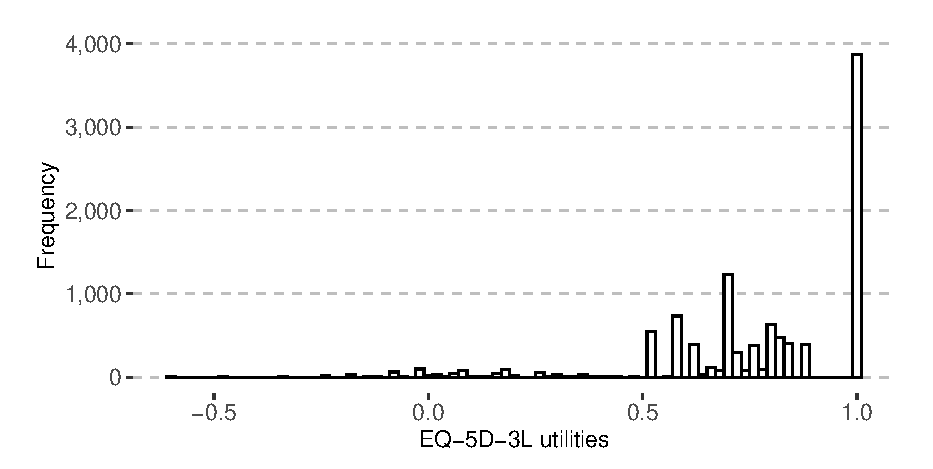
\includegraphics[keepaspectratio]{./plot_hist_obs.eps}}
\caption{\label{fig:plot-hist-obs} Frequency distribution of observed EQ-5D-3L utilities}
\end{figure}

\section{Examples}\label{examples}

\subsection{Model 1: Default settings}\label{sec:base}

We first fit model 1 with the default ``BFGS'' optimization method and ``zero'' initial values. The values 0.883 and -0.594 in the argument `psi' represent the maximum and minimum values smaller than 1 in the English value set (Dolan 1997). As the data shows a bi-modal distribution (figure \ref{fig:plot-hist-obs}), we estimate a mixture of 2 normal distributions (`ncmp' = 2). \texttt{aldvmm()} returns an object of class ``aldvmm''.

\begin{Shaded}
\begin{Highlighting}[]
\FunctionTok{library}\NormalTok{(}\StringTok{"aldvmm"}\NormalTok{)}

\NormalTok{fit }\OtherTok{\textless{}{-}}\NormalTok{ aldvmm}\SpecialCharTok{::}\FunctionTok{aldvmm}\NormalTok{(eq5d }\SpecialCharTok{\textasciitilde{}}\NormalTok{ hr }\SpecialCharTok{|} \DecValTok{1}\NormalTok{,}
                      \AttributeTok{data =}\NormalTok{ df,}
                      \AttributeTok{psi =} \FunctionTok{c}\NormalTok{(}\FloatTok{0.883}\NormalTok{, }\SpecialCharTok{{-}}\FloatTok{0.594}\NormalTok{),}
                      \AttributeTok{ncmp =} \DecValTok{2}\NormalTok{)}

\FunctionTok{summary}\NormalTok{(fit)}

\NormalTok{pred }\OtherTok{\textless{}{-}} \FunctionTok{predict}\NormalTok{(fit,}
                \AttributeTok{se.fit =} \ConstantTok{TRUE}\NormalTok{,}
                \AttributeTok{type =} \StringTok{"fit"}\NormalTok{)}
\end{Highlighting}
\end{Shaded}

We obtain a summary table of regression results using the generic function \texttt{summary()}. The model converges at a log-likelihood of -706 and an Akaike information criterion value of -1'399 (table \ref{tab:tab-sum-mod1bfgs}). The function \texttt{aldvmm()} returns the negative log-likelihood and Akaike information criterion, and smaller values suggest better fit.

The coefficients of the intercepts and covariates for the expected values \(E[y|c, X]\) of the normal distributions can be interpreted as marginal effects on component means. `lnsigma' denotes the natural logarithm of the estimated standard deviation \(\sigma^{c}\). The coefficients of covariates in the multinomial logit model of probabilities of component membership are log-transformed relative probabilities. Our model only includes two components, and the multinomial logit model collapses to a binomial logit model. The intercept of -0.728 means that the average probability of an observation in the data to belong to component 1 is \(\text{exp}(-0.728)\) or 0.4828738 times the probability to belong to component 2.

\begin{table}[ht]
\centering
\caption{Regression results from model 1 with "BFGS" optimization method and "zero" starting values} 
\label{tab:tab-sum-mod1bfgs}
\begin{tabular}{llrrrrrr}
  \hline
 &  & Estimate & Std. Error & t value & Pr($>$$|$t$|$) & 2.5 \% & 97.5 \% \\ 
  \hline
E[y$|$X, c] &  &  &  &  &  &  &  \\ 
   \hline
Comp1 & (Intercept) & -0.4307 & 0.0224 & -19.2351 & 0 & -0.4746 & -0.3868 \\ 
   & hr & 0.3135 & 0.0065 & 47.9498 & 0 & 0.3007 & 0.3263 \\ 
   & lnsigma & -1.2481 & 0.0215 & -58.0012 & 0 & -1.2903 & -1.2059 \\ 
  Comp2 & (Intercept) & 0.2358 & 0.0069 & 34.184 & 0 & 0.2223 & 0.2494 \\ 
   & hr & 0.1459 & 0.0019 & 76.3631 & 0 & 0.1421 & 0.1496 \\ 
   & lnsigma & -2.4624 & 0.0178 & -138.1263 & 0 & -2.4973 & -2.4274 \\ 
   \hline
P[c$|$X] &  &  &  &  &  &  &  \\ 
   \hline
Comp1 & (Intercept) & -0.728 & 0.0607 & -12.0018 & 0 & -0.8469 & -0.6091 \\ 
   \hline
N = 10549 & ll = -706 & AIC = -1399 & BIC = -1348 &  &  &  &  \\ 
  \end{tabular}
\end{table}

We obtain expected values of observations in the estimation data using the generic function \texttt{predict()}. Standard errors of fitted (estimation data) or predicted (new data) values are calculated using the delta method. Expected values exhibit a smoother distribution than observed values and do not show a gap between 1 and 0.883, because they are weighted averages of component distributions and 1 (figure \ref{fig:plot-hist-pred}).

\begin{figure}
\centering
\pandocbounded{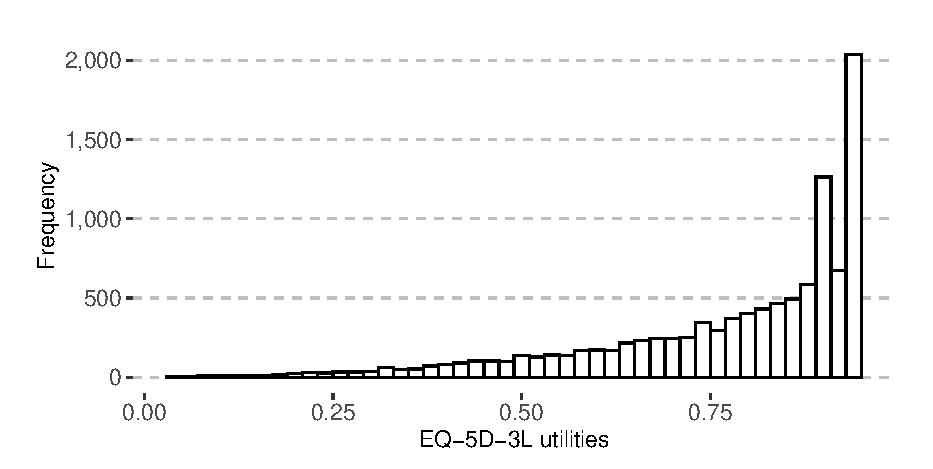
\includegraphics[keepaspectratio]{./plot_hist_pred.eps}}
\caption{\label{fig:plot-hist-pred} Expected values from base case model}
\end{figure}

Expected values of observations in the estimation data can also be used to calculate average incremental effects or average treatment effects on the treated. Average treatment effects on the treated compare predictions for treated individuals to predictions for the same individuals without the effect of the treatment indicator. Standard errors of average treatment effects on the treated can be calculated using the delta method (see example code in the \hyperref[atetcode]{appendix}).

A visual inspection of mean residuals over deciles of expected values (see example code of the modified Hosmer-Lemeshow test in the \hyperref[mhlcode]{appendix}) shows that model 1 fits the data poorly (figure \ref{fig:plot-comp-mhl-bfgs}). Although the test is overpowered with large data, and confidence bands should not be interpreted directly, the absolute over-prediction among individuals with low expected values is quite large.

\begin{figure}
\centering
\pandocbounded{\includegraphics[keepaspectratio]{./plot_comp_mhl_bfgs.eps}}
\caption{\label{fig:plot-comp-mhl-bfgs} Mean residuals over deciles of expected values, ``BFGS'' with ``zero'' starting values}
\end{figure}

We can use the `sandwich' package (Zeileis 2006) to calculate robust or clustered standard errors from objects of class ``aldvmm'' (see example code in the \hyperref[swcode]{appendix}).

\subsection{Model 1: Comparison of optimization methods}\label{model-1-comparison-of-optimization-methods}

Hernández Alava and Wailoo (2015) suggested that the likelihood function of the adjusted limited dependent variable mixture model with the English EQ-5D-3L data might have multiple local optima, and that the estimation is sensitive to initial values. We thus fit model 1 with all optimization algorithms and methods for generating initial values available in \texttt{aldvmm()} to assess the sensitivity of model fits to optimization settings and to find the maximum likelihood estimates.

\begin{Shaded}
\begin{Highlighting}[]
\NormalTok{init.method }\OtherTok{\textless{}{-}} \FunctionTok{c}\NormalTok{(}\StringTok{"zero"}\NormalTok{, }\StringTok{"random"}\NormalTok{, }\StringTok{"constant"}\NormalTok{, }\StringTok{"sann"}\NormalTok{)}

\NormalTok{optim.method }\OtherTok{\textless{}{-}} \FunctionTok{c}\NormalTok{(}\StringTok{"Nelder{-}Mead"}\NormalTok{, }\StringTok{"BFGS"}\NormalTok{, }\StringTok{"CG"}\NormalTok{, }\StringTok{"L{-}BFGS{-}B"}\NormalTok{, }\StringTok{"nlminb"}\NormalTok{, }\StringTok{"Rcgmin"}\NormalTok{, }
                  \StringTok{"Rvmmin"}\NormalTok{,}\StringTok{"hjn"}\NormalTok{)}

\NormalTok{fit1\_all }\OtherTok{\textless{}{-}} \FunctionTok{list}\NormalTok{()}

\ControlFlowTok{for}\NormalTok{ (i }\ControlFlowTok{in}\NormalTok{ init.method) \{}
  \ControlFlowTok{for}\NormalTok{ (j }\ControlFlowTok{in}\NormalTok{ optim.method) \{}
    \FunctionTok{set.seed}\NormalTok{(}\DecValTok{101010101}\NormalTok{) }\CommentTok{\# Seed for random starting values}
\NormalTok{    fit1\_all[[i]][[j]] }\OtherTok{\textless{}{-}}\NormalTok{ aldvmm}\SpecialCharTok{::}\FunctionTok{aldvmm}\NormalTok{(eq5d }\SpecialCharTok{\textasciitilde{}}\NormalTok{ hr }\SpecialCharTok{|} \DecValTok{1}\NormalTok{,}
                                         \AttributeTok{data         =}\NormalTok{ df,}
                                         \AttributeTok{psi          =} \FunctionTok{c}\NormalTok{(}\FloatTok{0.883}\NormalTok{, }\SpecialCharTok{{-}}\FloatTok{0.594}\NormalTok{),}
                                         \AttributeTok{ncmp         =} \DecValTok{2}\NormalTok{,}
                                         \AttributeTok{init.method  =}\NormalTok{ i,}
                                         \AttributeTok{optim.method =}\NormalTok{ j)}
\NormalTok{  \}}
\NormalTok{\}}
\end{Highlighting}
\end{Shaded}

The maximum likelihood varies considerably across optimization methods and initial values which confirms the sensitivity of the model to changes in these settings (table \ref{tab:ll}). The most frequent log-likelihood is 706.32, but the Hooke and Jeeves Pattern Search Optimization (``hjn'') with ``zero'' initial values converges at a log-likelihood 706.32.

The optimization methods ``Nelder-Mead'', ``CG'', ``L-BFGS-B'', ``Rcgmmin'' and ``hjn'' are particularly sensitive to changes of starting values. Only the method ``nlminb'' converges at the same log-likelihood of 706.32 regardless of initial values. However, even the ``nlminb'' algorithm converges at different parameters with starting values from a constant-only model than with the other starting values despite the same maximum log-likelihood.

\begin{table}[ht]
\centering
\caption{Log-likelihood by optimization method} 
\label{tab:ll}
\begin{tabular}{lrrrrrrrr}
  \hline
 & Nelder-Mead & BFGS & CG & L-BFGS-B & nlminb & Rcgmin & Rvmmin & hjn \\ 
  \hline
zero & -245.69 & 706.32 & -634.81 & -4513.33 & 706.32 & -634.81 & 706.32 & 706.32 \\ 
  random & 213.93 & -612.71 & 698.33 & -2830.18 & 706.32 & 706.32 & -606.34 & -627.78 \\ 
  constant & 706.32 & 706.32 & -634.81 & -634.81 & 706.32 & -634.81 & 706.32 & 706.32 \\ 
  sann & 706.32 & 706.32 & 698.67 & 706.32 & 706.32 & 706.32 & 706.32 & 706.32 \\ 
   \hline
\end{tabular}
\end{table}

The computation times of optimization routines were relatively short and did not vary considerably across methods expect for the ``hjn'' algorithm and simulated annealing ``sann'' starting values which requires more computation time (table \ref{tab:time}).

\begin{table}[ht]
\centering
\caption{Estimation time [minutes] by optimization method} 
\label{tab:time}
\begin{tabular}{lrrrrrrrr}
  \hline
 & Nelder-Mead & BFGS & CG & L-BFGS-B & nlminb & Rcgmin & Rvmmin & hjn \\ 
  \hline
zero & 0.42 & 0.10 & 0.16 & 0.06 & 0.11 & 0.11 & 0.09 & 1.71 \\ 
  random & 0.65 & 0.34 & 3.11 & 0.09 & 0.16 & 0.56 & 0.29 & 0.46 \\ 
  constant & 0.37 & 0.11 & 0.21 & 0.07 & 0.12 & 0.11 & 0.10 & 0.99 \\ 
  sann & 2.66 & 4.00 & 7.00 & 3.53 & 2.71 & 2.57 & 2.63 & 4.27 \\ 
   \hline
\end{tabular}
\end{table}

Parameter estimates differ considerably across selected optimization algorithms (table \ref{tab:tab-comp-coef}). The default ``BFGS'' - ``zero'' approach converges at the same parameters as the ``nlminb'' - ``zero'' method. The solution of the ``hjn'' method is rather extreme with no effect of the Oxford Hip Score, a very small standard deviation in component 2 and a very low probability of membership of component 2. Also, the Modified Hosmer-Lemeshow test did not show better fit of the ``hjn'' solution compared to the other algorithms (figure \ref{fig:plot-comp-mhl-nlminb} in the \hyperref[mhlres]{appendix}). The solution of the ``hjn'' method suggests that a single-component model should be explored as well.

\begin{table}[ht]
\centering
\caption{Regression results of model 1 with zero starting 
                     values in "BFGS", "Nelder-Mead", "nlminb" and "hjn" algorithms} 
\label{tab:tab-comp-coef}
\begin{tabular}{llrrrr}
  \hline
 &  & BFGS & Nelder-Mead & nlminb & hjn \\ 
  \hline
E[y$|$X, c] &  &  &  &  &  \\ 
   \hline
Comp1 & (Intercept) & -0.4307 & -0.0426 & -0.4307 & 0.2358 \\ 
   & hr & 0.3135 & 0.2194 & 0.3135 & 0.1459 \\ 
   & lnsigma & -1.2481 & -1.8595 & -1.2481 & -2.4624 \\ 
  Comp2 & (Intercept) & 0.2358 & 4.1853 & 0.2358 & -0.4307 \\ 
   & hr & 0.1459 & -1.0081 & 0.1459 & 0.3135 \\ 
   & lnsigma & -2.4624 & -0.0249 & -2.4624 & -1.2481 \\ 
   \hline
P[c$|$X] &  &  &  &  &  \\ 
   \hline
Comp1 & (Intercept) & -0.728 & 3.5636 & -0.728 & 0.728 \\ 
   \hline
ll &  & -706.32 & 245.69 & -706.32 & -706.32 \\ 
  \end{tabular}
\end{table}

As adjusted limited dependent variable mixture models are frequently used for tasks that rely on predictions, we also compare expected values from the ``BFGS'', ``Nelder-Mead'' and ``hjn'' methods to expected values from the ``nlminb'' method. Expected values from the ``Nelder-Mead'' method are smaller, and values from the ``hjn'' method are larger than ``nlminb'' values among observations with the lowest 80\% of expected values. Predictions from ``BFGS'' match predictions from the ``nlminb'' model fit closely (figure \ref{fig:plot-comp-pred}).

\begin{figure}
\centering
\pandocbounded{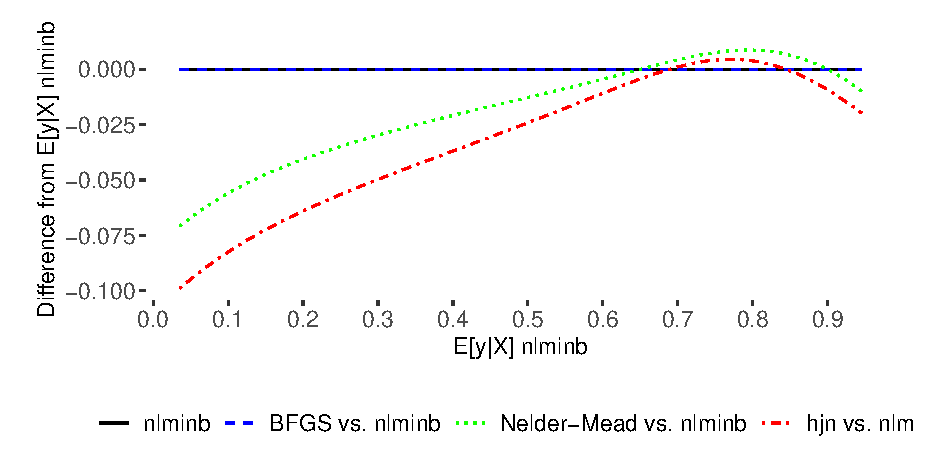
\includegraphics[keepaspectratio]{./plot_comp_pred.eps}}
\caption{\label{fig:plot-comp-pred} Deviation of expected values from ``BFGS'', ``Nelder-Mead'' and ``hjn'' versus ``nlminb'' with zero starting values}
\end{figure}

Based on the comparison of log-likelihoods, parameter estimates and predicted values, we deem the ``nlminb'' optimization method with ``zero'' starting values the most robust approach for the used data and model.

\subsection{Model 1: Constrained optimization with user-defined initial values}\label{model-1-constrained-optimization-with-user-defined-initial-values}

We can also fit model 1 with user-defined starting values and box constraints. When constraints are imposed, the \texttt{aldvmm()} function uses the optimization method ``L-BFGS-B'', which shows to be very sensitive to starting values. We use zero initial values for all parameters except for the intercept in the multinomial logit which we set to the estimate from the ``nlminb'' optimization method with ``zero'' starting values (0.7283) (table \ref{tab:tab-comp-coef}). We impose a lower limit of -3 to the log-standard deviations in both components.

The \texttt{aldvmm()} function returns a warning that the covariance matrix included negative values on the diagonal. We see that these values are the variances of the intercept and the log-standard deviation in component 2 (table \ref{tab:tab-sum-cstr}). The log-likelihood amounts to 628, which is smaller than the maximum log-likelihoods of model fits without constraints. The parameter estimates do not resemble any of the solutions of the unconstrained ``BFGS'', ``Nelder-Mead'', ``nlminb'' or ``hjn'' optimization methods with ``zero'' starting values (table \ref{tab:tab-comp-coef}), which further emphasizes the difficulties in finding a global optimum of the likelihood with English EQ-5D-3L utilities after hip replacement.

\begin{Shaded}
\begin{Highlighting}[]
\NormalTok{init }\OtherTok{\textless{}{-}} \FunctionTok{c}\NormalTok{(}\DecValTok{0}\NormalTok{,    }\DecValTok{0}\NormalTok{,   }\DecValTok{0}\NormalTok{,   }\DecValTok{0}\NormalTok{,    }\DecValTok{0}\NormalTok{,    }\DecValTok{0}\NormalTok{,    }\FloatTok{0.7283}\NormalTok{)}
\NormalTok{lo   }\OtherTok{\textless{}{-}} \FunctionTok{c}\NormalTok{(}\SpecialCharTok{{-}}\ConstantTok{Inf}\NormalTok{, }\SpecialCharTok{{-}}\ConstantTok{Inf}\NormalTok{, }\SpecialCharTok{{-}}\DecValTok{3}\NormalTok{,  }\SpecialCharTok{{-}}\ConstantTok{Inf}\NormalTok{, }\SpecialCharTok{{-}}\ConstantTok{Inf}\NormalTok{, }\SpecialCharTok{{-}}\DecValTok{3}\NormalTok{, }\SpecialCharTok{{-}}\ConstantTok{Inf}\NormalTok{)}
\NormalTok{hi   }\OtherTok{\textless{}{-}} \FunctionTok{c}\NormalTok{(}\ConstantTok{Inf}\NormalTok{,  }\ConstantTok{Inf}\NormalTok{,  }\ConstantTok{Inf}\NormalTok{, }\ConstantTok{Inf}\NormalTok{,  }\ConstantTok{Inf}\NormalTok{,  }\ConstantTok{Inf}\NormalTok{,  }\ConstantTok{Inf}\NormalTok{)}

\NormalTok{fit1\_cstr }\OtherTok{\textless{}{-}}\NormalTok{ aldvmm}\SpecialCharTok{::}\FunctionTok{aldvmm}\NormalTok{(eq5d }\SpecialCharTok{\textasciitilde{}}\NormalTok{ hr }\SpecialCharTok{|} \DecValTok{1}\NormalTok{,}
                            \AttributeTok{data =}\NormalTok{ df,}
                            \AttributeTok{psi =} \FunctionTok{c}\NormalTok{(}\FloatTok{0.883}\NormalTok{, }\SpecialCharTok{{-}}\FloatTok{0.594}\NormalTok{),}
                            \AttributeTok{ncmp =} \DecValTok{2}\NormalTok{,}
                            \AttributeTok{init.est =}\NormalTok{ init,}
                            \AttributeTok{init.lo =}\NormalTok{ lo,}
                            \AttributeTok{init.hi =}\NormalTok{ hi)}

\FunctionTok{summary}\NormalTok{(fit1\_cstr)}
\end{Highlighting}
\end{Shaded}

\begin{table}[ht]
\centering
\caption{Regression results of model 1 with the "L-BFGS-B" method, parameter constraints and user-defined starting values} 
\label{tab:tab-sum-cstr}
\begin{tabular}{llrrrrrr}
  \hline
 &  & Estimate & Std. Error & t value & Pr($>$$|$t$|$) & 2.5 \% & 97.5 \% \\ 
  \hline
E[y$|$X, c] &  &  &  &  &  &  &  \\ 
   \hline
Comp1 & (Intercept) & -0.092 & 0.0085 & -10.8048 & 0 & -0.1087 & -0.0753 \\ 
   & hr & 0.2325 & 0.0023 & 101.8493 & 0 & 0.228 & 0.237 \\ 
   & lnsigma & -1.6406 & 0.0089 & -183.9809 & 0 & -1.6581 & -1.6231 \\ 
  Comp2 & (Intercept) & 0.3931 & NaN & NaN & NaN & NaN & NaN \\ 
   & hr & 2.5249 & 7.4795 & 0.3376 & 0.7357 & -12.1363 & 17.1861 \\ 
   & lnsigma & -0.7651 & NaN & NaN & NaN & NaN & NaN \\ 
   \hline
P[c$|$X] &  &  &  &  &  &  &  \\ 
   \hline
Comp1 & (Intercept) & 6.852 & 0.5388 & 12.7168 & 0 & 5.7958 & 7.9082 \\ 
   \hline
N = 10549 & ll = 628 & AIC = 1270 & BIC = 1320 &  &  &  &  \\ 
  \end{tabular}
\end{table}

\subsection{Model 1: Single-component model}\label{model-1-single-component-model}

As the solution of the ``hjn'' algorithm includes a component with very low probability, we also estimate a single-component model.

\begin{Shaded}
\begin{Highlighting}[]
\NormalTok{fit }\OtherTok{\textless{}{-}}\NormalTok{ aldvmm}\SpecialCharTok{::}\FunctionTok{aldvmm}\NormalTok{(eq5d }\SpecialCharTok{\textasciitilde{}}\NormalTok{ hr,}
                      \AttributeTok{data =}\NormalTok{ df,}
                      \AttributeTok{psi =} \FunctionTok{c}\NormalTok{(}\FloatTok{0.883}\NormalTok{, }\SpecialCharTok{{-}}\FloatTok{0.594}\NormalTok{),}
                      \AttributeTok{ncmp =} \DecValTok{1}\NormalTok{,}
                      \AttributeTok{init.method =} \StringTok{"zero"}\NormalTok{,}
                      \AttributeTok{optim.method =} \StringTok{"nlminb"}\NormalTok{)}

\FunctionTok{summary}\NormalTok{(fit)}
\end{Highlighting}
\end{Shaded}

The coefficients of the single-component model are relatively similar to the parameters in the second component of model 1 from the ``hjn'' algorithm (table \ref{tab:tab-sum-tobit}). The Akaike information criterion amounts to 1'276 which is larger than the values of the ``nlminb'' (-706.32) and ``hjn'' (-706.32) solutions of the two-component model and thus suggests worse fit of the single-component model.\footnote{In the `aldvmm()` output, smaller values of the Akaike information criterion indicate better goodness of fit.}

\begin{table}[ht]
\centering
\caption{Regression results of model 1 with 1 component, 
                     zero starting values in "nlminb" algorithm} 
\label{tab:tab-sum-tobit}
\begin{tabular}{llrrrrrr}
  \hline
 &  & Estimate & Std. Error & t value & Pr($>$$|$t$|$) & 2.5 \% & 97.5 \% \\ 
  \hline
E[y$|$X, c] &  &  &  &  &  &  &  \\ 
   \hline
Comp1 & (Intercept) & -0.0886 & 0.0085 & -10.4099 & 0 & -0.1053 & -0.0719 \\ 
   & hr & 0.2318 & 0.0023 & 101.4681 & 0 & 0.2273 & 0.2362 \\ 
   & lnsigma & -1.6363 & 0.0089 & -184.2422 & 0 & -1.6537 & -1.6189 \\ 
   \hline
N = 10549 & ll = 635 & AIC = 1276 & BIC = 1297 &  &  &  &  \\ 
  \end{tabular}
\end{table}

\subsection{Model 2: User-defined starting values}\label{model-2-user-defined-starting-values}

As an alternative specification, we explore model 2 with a coefficient of the Oxford Hip score in the multinomial logit model of component membership. For this fit, we use the method ``nlminb'' with estimates from Hernández Alava and Wailoo (2015) as starting values.

\begin{Shaded}
\begin{Highlighting}[]
\NormalTok{init }\OtherTok{\textless{}{-}} \FunctionTok{c}\NormalTok{(}\SpecialCharTok{{-}}\NormalTok{.}\DecValTok{40293118}\NormalTok{, .}\DecValTok{30502755}\NormalTok{, .}\DecValTok{22614716}\NormalTok{, .}\DecValTok{14801581}\NormalTok{, }\SpecialCharTok{{-}}\NormalTok{.}\DecValTok{70755741}\NormalTok{, }\DecValTok{0}\NormalTok{, }
          \SpecialCharTok{{-}}\FloatTok{1.2632051}\NormalTok{, }\SpecialCharTok{{-}}\FloatTok{2.4541401}\NormalTok{)}

\NormalTok{fit2 }\OtherTok{\textless{}{-}}\NormalTok{ aldvmm}\SpecialCharTok{::}\FunctionTok{aldvmm}\NormalTok{(eq5d }\SpecialCharTok{\textasciitilde{}}\NormalTok{ hr }\SpecialCharTok{|}\NormalTok{ hr,}
                       \AttributeTok{data =}\NormalTok{ df,}
                       \AttributeTok{psi =} \FunctionTok{c}\NormalTok{(}\FloatTok{0.883}\NormalTok{, }\SpecialCharTok{{-}}\FloatTok{0.594}\NormalTok{),}
                       \AttributeTok{ncmp =} \DecValTok{2}\NormalTok{,}
                       \AttributeTok{init.est =}\NormalTok{ init,}
                       \AttributeTok{optim.method =} \StringTok{"nlminb"}\NormalTok{)}

\FunctionTok{summary}\NormalTok{(fit2)}
\end{Highlighting}
\end{Shaded}

The Akaike information criterion of model 2 fitted using the ``nlminb'' method amounts to -1'867 which is smaller than the Akaike information criterion of model 1 (-706.32) with the same method. The smaller Akaike information criterion suggests that the increase in the log-likelihood after inclusion of a coefficient of the Oxford Hip Score on the probability of component membership is sufficiently large to justify the extra parameter.\footnote{In the `aldvmm()` output, smaller values of the Akaike information criterion indicate better goodness of fit.}

\begin{table}[ht]
\centering
\caption{Regression results of model 2 with user-defined 
                     starting values in the "nlminb" algorithm} 
\label{tab:tab-sum-mod2}
\begin{tabular}{llrrrrrr}
  \hline
 &  & Estimate & Std. Error & t value & Pr($>$$|$t$|$) & 2.5 \% & 97.5 \% \\ 
  \hline
E[y$|$X, c] &  &  &  &  &  &  &  \\ 
   \hline
Comp1 & (Intercept) & 0.0031 & 0.0281 & 0.1085 & 0.9136 & -0.0521 & 0.0582 \\ 
   & hr & 0.0965 & 0.0116 & 8.352 & 0 & 0.0739 & 0.1192 \\ 
   & lnsigma & -1.2676 & 0.0314 & -40.4144 & 0 & -1.3291 & -1.2061 \\ 
  Comp2 & (Intercept) & 0.1816 & 0.0074 & 24.5104 & 0 & 0.1671 & 0.1961 \\ 
   & hr & 0.1609 & 0.0019 & 85.4201 & 0 & 0.1573 & 0.1646 \\ 
   & lnsigma & -2.2809 & 0.0126 & -181.079 & 0 & -2.3056 & -2.2563 \\ 
   \hline
P[c$|$X] &  &  &  &  &  &  &  \\ 
   \hline
Comp1 & (Intercept) & 2.4455 & 0.1719 & 14.2293 & 0 & 2.1086 & 2.7824 \\ 
   & hr & -1.3902 & 0.0566 & -24.5697 & 0 & -1.5011 & -1.2793 \\ 
   \hline
N = 10549 & ll = -941 & AIC = -1867 & BIC = -1809 &  &  &  &  \\ 
  \end{tabular}
\end{table}

\section{\texorpdfstring{Comparison to STATA\textsuperscript{\textregistered} results}{Comparison to STATA results}}\label{comparison-to-stata-results}

To validate the R implementation of adjusted limited dependent variable mixture models, we estimate the four models presented in Hernández Alava and Wailoo (2015) as reference cases in R and STATA\textsuperscript{\textregistered}.\footnote{The STATA\textsuperscript{\textregistered} and R code for model estimation is included in the [appendix](#rcode).}

\begin{enumerate}
\def\labelenumi{\arabic{enumi}.}
\item
  Model 1 with default options
\item
  Model 1 with parameter constraints
\item
  Model 1 with initial values from constant-only model
\item
  Model 2 with user-defined initial values
\end{enumerate}

The parameter estimates and standard errors obtained in R are very similar to the results from STATA\textsuperscript{\textregistered} (table \ref{tab:tab-comp-stata} and table \ref{tab:tab-compse-stata}). R did not obtain any standard errors in reference model 2 while STATA\textsuperscript{\textregistered} returns standard errors for the first component and the probability of belonging to component 1. Although reference models 1 and 3 yield different parameter estimates, they converge at the same log-likelihood which further supports the hypothesis of multiple local optima of the likelihood. The relative ordering of models is consistent across platforms.

\begin{table}[ht]
\centering
\caption{Comparison of point estimates to the results of the STATA package} 
\label{tab:tab-comp-stata}
\begin{tabular}{llrrrrrrrr}
  \hline
  &  & (1) &  & (2) &  & (3) &  & (4) &  \\ 
   &  & R & STATA & R & STATA & R & STATA & R & STATA \\ 
   \hline
E[y$|$X, c] &  &  &  &  &  &  &  &  &  \\ 
   \hline
Comp1 & (Intercept) & -0.4307 & -0.427 & -0.092 & -0.092 & 0.2358 & 0.236 & 0.0031 & 0.006 \\ 
   & hr & 0.3135 & 0.312 & 0.2325 & 0.232 & 0.1459 & 0.146 & 0.0965 & 0.095 \\ 
   & lnsigma & -1.2481 & -1.251 & -1.6406 & -1.641 & -2.4624 & -2.463 & -1.2676 & -1.274 \\ 
  Comp2 & (Intercept) & 0.2358 & 0.236 & 100 & 100.000 & -0.4307 & -0.427 & 0.1816 & 0.182 \\ 
   & hr & 0.1459 & 0.146 & 0 & 0.000 & 0.3135 & 0.312 & 0.1609 & 0.161 \\ 
   & lnsigma & -2.4624 & -2.463 & 0 & 0.000 & -1.2481 & -1.251 & -2.2809 & -2.280 \\ 
   \hline
P[c$|$X] &  &  &  &  &  &  &  &  &  \\ 
   \hline
Comp1 & (Intercept) & -0.728 & -0.725 & 6.8564 & 6.855 & 0.728 & 0.725 & 2.4455 & 2.448 \\ 
   & hr &  &  &  &  &  &  & -1.3902 & -1.393 \\ 
   \hline
N = 10549 & ll & -706 & 715.84 & 628 & -613.7 & -706 & 715.84 & -941 & 953.2 \\ 
  \end{tabular}
\end{table}
\begin{table}[!ht]
\centering
\caption{Comparison of standard errors to the results of the STATA package.} 
\label{tab:tab-compse-stata}
\begin{tabular}{llrrrrrrrr}
  \hline
  &  & (1) &  & (2) &  & (3) &  & (4) &  \\ 
   &  & R & STATA & R & STATA & R & STATA & R & STATA \\ 
   \hline
E[y$|$X, c] &  &  &  &  &  &  &  &  &  \\ 
   \hline
Comp1 & (Intercept) & 0.0224 & 0.022 & NA & 0.009 & 0.0069 & 0.007 & 0.0281 & 0.028 \\ 
   & hr & 0.0065 & 0.006 & NA & 0.002 & 0.0019 & 0.002 & 0.0116 & 0.012 \\ 
   & lnsigma & 0.0215 & 0.021 & NA & 0.009 & 0.0178 & -0.018 & 0.0314 & 0.032 \\ 
  Comp2 & (Intercept) & 0.0069 & 0.007 & NA &  & 0.0224 & 0.022 & 0.0074 & 0.007 \\ 
   & hr & 0.0019 & 0.002 & NA &  & 0.0065 & 0.006 & 0.0019 & 0.002 \\ 
   & lnsigma & 0.0178 & 0.018 & NA &  & 0.0215 & 0.021 & 0.0126 & 0.013 \\ 
   \hline
P[c$|$X] &  &  &  &  &  &  &  &  &  \\ 
   \hline
Comp1 & (Intercept) & 0.0607 & 0.061 & NA & 0.540 & 0.0607 & 0.061 & 0.1719 & 0.172 \\ 
   & hr &  &  &  &  &  &  & 0.0566 & 0.056 \\ 
   \hline
N = 10549 & ll & -706 & 715.84 & 628 & -613.7 & -706 & 715.84 & -941 & 953.2 \\ 
  \end{tabular}
\end{table}

Fitted values show very similar marginal distributions on both platforms (figure \ref{fig:box-pred-yhat-stata}). R does not return fitted values in reference case 2. The summary statistics of differences in fitted values between R and STATA\textsuperscript{\textregistered} suggest that individual predictions are quite similar across platforms as well (table \ref{tab:compyhat}).

Standard errors of fitted values differ visibly between platforms (figure \ref{fig:box-pred-se-stata} and table \ref{tab:compse}). The difference is particularly pronounced in reference case 1, but the standard errors from STATA\textsuperscript{\textregistered} seem quite extreme compared to all other reference cases. R does not return standard errors of fitted values in reference case 2.

\begin{figure}
\centering
\pandocbounded{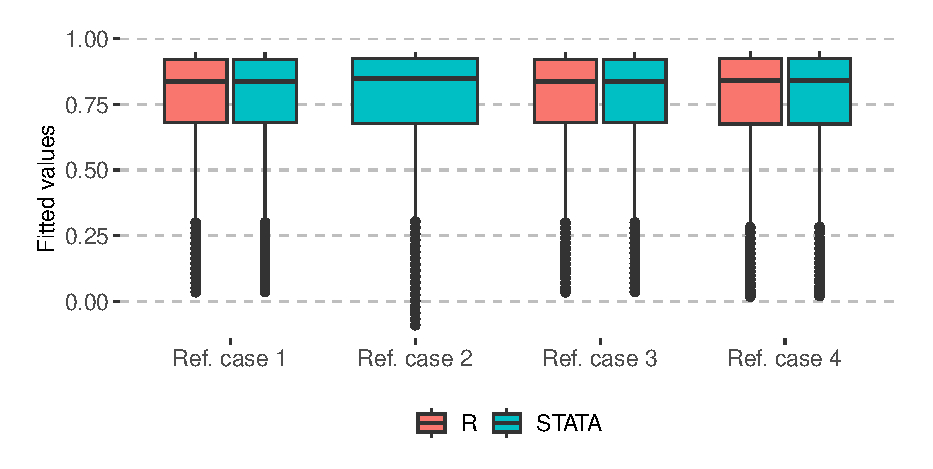
\includegraphics[keepaspectratio]{./plot_box_yhat.eps}}
\caption{\label{fig:box-pred-yhat-stata} Fitted values in R and STATA}
\end{figure}

\begin{figure}
\centering
\pandocbounded{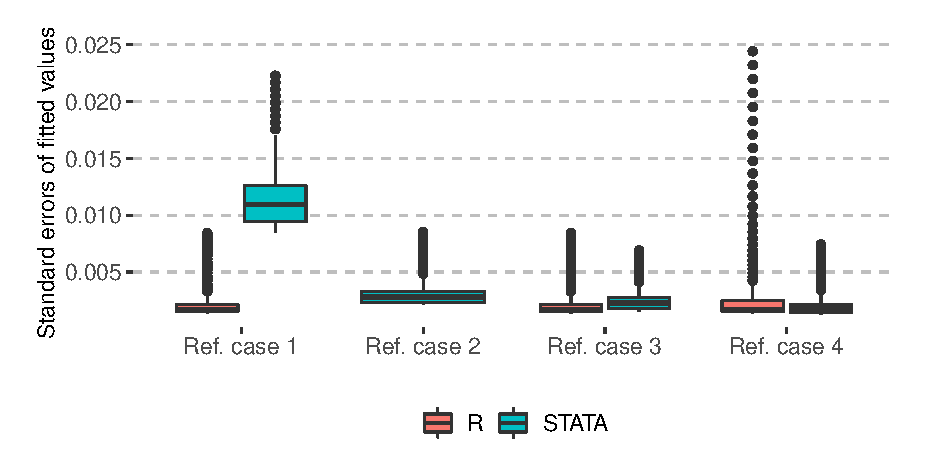
\includegraphics[keepaspectratio]{./plot_box_se.eps}}
\caption{\label{fig:box-pred-se-stata} Standard errors of fitted values in R and STATA}
\end{figure}

\begin{table}[ht]
\centering
\caption{Summary statistics of differences of fitted values in R and STATA (positive values suggest larger values in STATA)} 
\label{tab:compyhat}
\begin{tabular}{lrrrr}
  \hline
 & Ref. case 1 & Ref. case 2 & Ref. case 3 & Ref. case 4 \\ 
  \hline
Min. & -0.000038 &  & -0.000038 & -0.000051 \\ 
  1st Qu. & -0.000036 &  & -0.000036 & -0.000044 \\ 
  Median & -0.000033 &  & -0.000033 & 0.000008 \\ 
  Mean & 0.000037 &  & 0.000037 & 0.000035 \\ 
  3rd Qu. & 0.000047 &  & 0.000047 & 0.000070 \\ 
  Max. & 0.000567 &  & 0.000567 & 0.002319 \\ 
   \hline
\end{tabular}
\end{table}

\begin{table}[ht]
\centering
\caption{Summary statistics of differences of standard errors of fitted values in R and STATA (positive values suggest larger values in STATA)} 
\label{tab:compse}
\begin{tabular}{lrrrr}
  \hline
 & Ref. case 1 & Ref. case 2 & Ref. case 3 & Ref. case 4 \\ 
  \hline
Min. & 0.005897 &  & -0.002063 & -0.016984 \\ 
  1st Qu. & 0.006898 &  & -0.000551 & -0.000823 \\ 
  Median & 0.008690 &  & 0.000189 & -0.000364 \\ 
  Mean & 0.008917 &  & 0.000171 & -0.000515 \\ 
  3rd Qu. & 0.011050 &  & 0.001054 & 0.000354 \\ 
  Max. & 0.013830 &  & 0.001530 & 0.000792 \\ 
   \hline
\end{tabular}
\end{table}

The comparison of the R and STATA\textsuperscript{\textregistered} packages shows that the R implementation sometimes behaves differently than the STATA\textsuperscript{\textregistered} package, but the results are not indicative of technical errors in the R implementation.

\section{Discussion}\label{discussion}

Adjusted limited dependent variable mixture models are powerful tools for regression analysis of health state utilities. Unlike standard regression models, adjusted limited dependent variable mixture models account for limits, gaps and multi-modal distributions.

The comparison of different optimization methods with EQ-5D-3L utility data from English patients after hip replacement in 2011 and 2012 (NHS Digital 2013) showed that the likelihood function can be challenging to maximize and can converge at local optima or extreme solutions. Parameter estimates varied considerably across optimization methods and even across methods with the same maximum log-likelihood. However, fitted values were very similar across the four reference cases which suggests that the model is more robust for the identification of incremental and average marginal effects than for parameter identification.

The `aldvmm' package offers a variety of optimization algorithms and methods for generating initial values which is an important strength in such challenging situations. It is essential to assess different optimization algorithms and methods for initial values before interpreting the parameter estimates or predictions of adjusted limited dependent variable mixture models.

The analysis of the EQ-5D-3L utility data also suggests that simpler models with fewer components should be considered when multi-component models are difficult to fit. Even single-component adjusted limited dependent variable mixture models can improve fit compared to traditional regression techniques because they account for limits and gaps.

Although coefficients can be interpreted as marginal effects within each component, they cannot be interpreted in terms of overall expected values. Thus, average marginal effects and average treatment effects need to be calculated from predictions using the generic function \texttt{predict()}. Standard errors of marginal effects or average treatment effects can be calculated using the delta method.

When no valid covariance matrix of parameters can be obtained or the user is in doubt of the validity of standard errors, the function \texttt{sandwich::vcovBS()} can be used to obtain bootstrapped standard errors. Due to the large variability of results across model fits, a large number of iterations might be needed which increases computation time. Other functions from the `sandwich' package can also be used to estimate robust or clustered standard errors.

In situations with repeated utility measures, the `aldvmm' package only allows fixed effects estimations with group and time fixed effects which can be an important limitation in the analysis of clinical data. However, time fixed effects can be an appropriate modeling strategy in the presence of general time trends and dynamic selection in the population, e.g.~because health state utilities decrease over time and treated individuals survive longer and thus are over-represented in later measurements.

Possible extensions of the `aldvmm' package could include additional component distributions, a mixed model implementation for repeated measures and an implementation of functions for calculating average marginal effects and their standard errors.

\newpage

\section*{References}\label{references}
\addcontentsline{toc}{section}{References}

\phantomsection\label{refs}
\begin{CSLReferences}{1}{0}
\bibitem[\citeproctext]{ref-Dixon2020}
Dixon, Padraig, William Hollingworth, and John Sparrow. 2020. {``Mapping to Quality of Life and Capability Measures in Cataract Surgery Patients: From Cat-PROM5 to EQ-5D-3L, EQ-5D-5L, and ICECAP-o Using Mixture Modelling.''} \emph{MDM Policy \& Practice} 5 (1): 2381468320915447.

\bibitem[\citeproctext]{ref-Dolan1997}
Dolan, Paul. 1997. {``Modeling Valuations for EuroQol Health States.''} \emph{Medical Care}, 1095--1108.

\bibitem[\citeproctext]{ref-Dowd2014}
Dowd, Bryan E, William H Greene, and Edward C Norton. 2014. {``Computation of Standard Errors.''} \emph{Health Services Research} 49 (2): 731--50.

\bibitem[\citeproctext]{ref-Fuller2017}
Fuller, Gordon Ward, Monica Hernandez, David Pallot, Fiona Lecky, Mathew Stevenson, and Belinda Gabbe. 2017. {``Health State Preference Weights for the Glasgow Outcome Scale Following Traumatic Brain Injury: A Systematic Review and Mapping Study.''} \emph{Value in Health} 20 (1): 141--51.

\bibitem[\citeproctext]{ref-Gray2018}
Gray, Laura A, Mónica Hernández Alava, and Allan J Wailoo. 2018. {``Development of Methods for the Mapping of Utilities Using Mixture Models: Mapping the AQLQ-s to the EQ-5D-5L and the HUI3 in Patients with Asthma.''} \emph{Value in Health} 21 (6): 748--57.

\bibitem[\citeproctext]{ref-Gray2018a}
Gray, Laura A, Allan J Wailoo, and Mónica Hernández Alava. 2018. {``Mapping the FACT-b Instrument to EQ-5D-3L in Patients with Breast Cancer Using Adjusted Limited Dependent Variable Mixture Models Versus Response Mapping.''} \emph{Value in Health} 21 (12): 1399--1405.

\bibitem[\citeproctext]{ref-HernandezAlava2015}
Hernández Alava, Mónica, and Allan Wailoo. 2015. {``Fitting Adjusted Limited Dependent Variable Mixture Models to {EQ-5D}.''} \emph{The Stata Journal} 15 (3): 737--50.

\bibitem[\citeproctext]{ref-HernandezAlava2012}
Hernández Alava, Mónica, Allan J Wailoo, and Roberta Ara. 2012. {``Tails from the Peak District: Adjusted Limited Dependent Variable Mixture Models of {EQ-5D} Questionnaire Health State Utility Values.''} \emph{Value in Health} 15 (3): 550--61.

\bibitem[\citeproctext]{ref-HernandezAlava2013}
Hernández Alava, Mónica, Allan Wailoo, Fred Wolfe, and Kaleb Michaud. 2013. {``The Relationship Between {EQ-5D}, {HAQ} and Pain in Patients with Rheumatoid Arthritis.''} \emph{Rheumatology} 52 (5): 944--50.

\bibitem[\citeproctext]{ref-HernandezAlava2014}
---------. 2014. {``A Comparison of Direct and Indirect Methods for the Estimation of Health Utilities from Clinical Outcomes.''} \emph{Medical Decision Making} 34 (7): 919--30.

\bibitem[\citeproctext]{ref-Mukuria2019}
Mukuria, Clara, Donna Rowen, Sue Harnan, Andrew Rawdin, Ruth Wong, Roberta Ara, and John Brazier. 2019. {``An Updated Systematic Review of Studies Mapping (or Cross-Walking) Measures of Health-Related Quality of Life to Generic Preference-Based Measures to Generate Utility Values.''} \emph{Applied Health Economics and Health Policy}, 1--19.

\bibitem[\citeproctext]{ref-Mulhern2018}
Mulhern, Brendan, Yan Feng, Koonal Shah, Mathieu F Janssen, Michael Herdman, Ben van Hout, and Nancy Devlin. 2018. {``Comparing the UK EQ-5D-3L and English EQ-5D-5L Value Sets.''} \emph{Pharmacoeconomics} 36 (6): 699--713.

\bibitem[\citeproctext]{ref-NHSDigital2013}
NHS Digital. 2013. {``Finalised Patient Reported Outcome Measures (PROMs) in England - April 2011 to March 2012. Patient Reported Outcome Measures (PROMs).''} \emph{Https://Digital.nhs.uk/Data-and-Information/Publications/Statistical/Patient-Reported-Outcome-Measures-Proms/Finalised-Patient-Reported-Outcome-Measures-Proms-in-England-April-2011-to-March-2012} October 15, 2013.

\bibitem[\citeproctext]{ref-Pennington2020}
Pennington, Becky M, Mónica Hernández Alava, Philip Hykin, Sobha Sivaprasad, Laura Flight, Abualbishr Alshreef, and John Brazier. 2020. {``Mapping from Visual Acuity to EQ-5D, EQ-5D with Vision Bolt-on, and VFQ-UI in Patients with Macular Edema in the LEAVO Trial.''} \emph{Value in Health} 23 (7): 928--35.

\bibitem[\citeproctext]{ref-Whitmore1986}
Whitmore, GA. 1986. {``Prediction Limits for a Univariate Normal Observation.''} \emph{The American Statistician} 40 (2): 141--43.

\bibitem[\citeproctext]{ref-Xu2020}
Xu, Richard Huan, Eliza Lai Yi Wong, Jun Jin, Ying Dou, and Dong Dong. 2020. {``Mapping of the EORTC QLQ-C30 to EQ-5D-5L Index in Patients with Lymphomas.''} \emph{The European Journal of Health Economics} 21 (9): 1363--73.

\bibitem[\citeproctext]{ref-Yang2019}
Yang, Fan, Carlos KH Wong, Nan Luo, James Piercy, Rebecca Moon, and James Jackson. 2019. {``Mapping the Kidney Disease Quality of Life 36-Item Short Form Survey (KDQOL-36) to the EQ-5D-3L and the EQ-5D-5L in Patients Undergoing Dialysis.''} \emph{The European Journal of Health Economics} 20 (8): 1195--1206.

\bibitem[\citeproctext]{ref-Zeileis2006}
Zeileis, Achim. 2006. {``Object-Oriented Computation of Sandwich Estimators.''} \emph{Journal of Statistical Software} 16 (9): 1--16. \url{https://doi.org/10.18637/jss.v016.i09}.

\end{CSLReferences}

\newpage

\section*{Appendix}\label{appendix}
\addcontentsline{toc}{section}{Appendix}

\subsection*{Example calculation of average treatment effects on the treated}\label{atetcode}

\begin{Shaded}
\begin{Highlighting}[]
\CommentTok{\# Create treatment indicator}
\CommentTok{\#{-}{-}{-}{-}{-}{-}{-}{-}{-}{-}{-}{-}{-}{-}{-}{-}{-}{-}{-}{-}{-}{-}{-}{-}{-}{-}{-}}

\NormalTok{df}\SpecialCharTok{$}\NormalTok{treated }\OtherTok{\textless{}{-}} \FunctionTok{as.numeric}\NormalTok{(df}\SpecialCharTok{$}\NormalTok{SEX }\SpecialCharTok{==} \StringTok{"2"}\NormalTok{)}

\CommentTok{\# Fit model}
\CommentTok{\#{-}{-}{-}{-}{-}{-}{-}{-}{-}{-}}

\NormalTok{formula }\OtherTok{\textless{}{-}}\NormalTok{ eq5d }\SpecialCharTok{\textasciitilde{}}\NormalTok{ treated }\SpecialCharTok{+}\NormalTok{ hr }\SpecialCharTok{|} \DecValTok{1}

\NormalTok{fit }\OtherTok{\textless{}{-}} \FunctionTok{aldvmm}\NormalTok{(formula,}
              \AttributeTok{data =}\NormalTok{ df,}
              \AttributeTok{psi =} \FunctionTok{c}\NormalTok{(}\SpecialCharTok{{-}}\FloatTok{0.594}\NormalTok{, }\FloatTok{0.883}\NormalTok{))}

\CommentTok{\# Predict treated}
\CommentTok{\#{-}{-}{-}{-}{-}{-}{-}{-}{-}{-}{-}{-}{-}{-}{-}{-}}

\CommentTok{\# Subsample of treated observations}
\NormalTok{tmpdf1 }\OtherTok{\textless{}{-}}\NormalTok{ df[df}\SpecialCharTok{$}\NormalTok{treated }\SpecialCharTok{==} \DecValTok{1}\NormalTok{, ]}

\CommentTok{\# Design matrix for treated observations}
\NormalTok{X1 }\OtherTok{\textless{}{-}} \FunctionTok{aldvmm.mm}\NormalTok{(}\AttributeTok{data =}\NormalTok{ tmpdf1,}
                \AttributeTok{formula =}\NormalTok{ fit}\SpecialCharTok{$}\NormalTok{formula,}
                \AttributeTok{ncmp =}\NormalTok{ fit}\SpecialCharTok{$}\NormalTok{k,}
                \AttributeTok{lcoef =}\NormalTok{ fit}\SpecialCharTok{$}\NormalTok{label}\SpecialCharTok{$}\NormalTok{lcoef)}

\CommentTok{\# Average expected outcome of treated observations}
\NormalTok{mean1 }\OtherTok{\textless{}{-}} \FunctionTok{mean}\NormalTok{(}\FunctionTok{predict}\NormalTok{(fit,}
                      \AttributeTok{newdata =}\NormalTok{ tmpdf1,}
                      \AttributeTok{type =} \StringTok{"fit"}\NormalTok{,}
                      \AttributeTok{se.fit =} \ConstantTok{TRUE}\NormalTok{)[[}\StringTok{"yhat"}\NormalTok{]], }\AttributeTok{na.rm =} \ConstantTok{TRUE}\NormalTok{)}

\CommentTok{\# Predict counterfactual}
\CommentTok{\#{-}{-}{-}{-}{-}{-}{-}{-}{-}{-}{-}{-}{-}{-}{-}{-}{-}{-}{-}{-}{-}{-}{-}}

\CommentTok{\# Subsample of counterfactual observations}
\NormalTok{tmpdf0 }\OtherTok{\textless{}{-}}\NormalTok{ tmpdf1}
\FunctionTok{rm}\NormalTok{(tmpdf1)}
\NormalTok{tmpdf0}\SpecialCharTok{$}\NormalTok{treated }\OtherTok{\textless{}{-}} \DecValTok{0}

\CommentTok{\# Design matrix for counterfactual observations}
\NormalTok{X0 }\OtherTok{\textless{}{-}} \FunctionTok{aldvmm.mm}\NormalTok{(}\AttributeTok{data =}\NormalTok{ tmpdf0,}
                \AttributeTok{formula =}\NormalTok{ fit}\SpecialCharTok{$}\NormalTok{formula,}
                \AttributeTok{ncmp =}\NormalTok{ fit}\SpecialCharTok{$}\NormalTok{k,}
                \AttributeTok{lcoef =}\NormalTok{ fit}\SpecialCharTok{$}\NormalTok{label}\SpecialCharTok{$}\NormalTok{lcoef)}

\CommentTok{\# Average expected outcome of counterfactual osbervations}
\NormalTok{mean0 }\OtherTok{\textless{}{-}} \FunctionTok{mean}\NormalTok{(}\FunctionTok{predict}\NormalTok{(fit,}
                      \AttributeTok{newdata =}\NormalTok{ tmpdf0,}
                      \AttributeTok{type =} \StringTok{"fit"}\NormalTok{,}
                      \AttributeTok{se.fit =} \ConstantTok{TRUE}\NormalTok{)[[}\StringTok{"yhat"}\NormalTok{]], }\AttributeTok{na.rm =} \ConstantTok{TRUE}\NormalTok{)}

\FunctionTok{rm}\NormalTok{(tmpdf0)}

\CommentTok{\# Standard error of ATET}
\CommentTok{\#{-}{-}{-}{-}{-}{-}{-}{-}{-}{-}{-}{-}{-}{-}{-}{-}{-}{-}{-}{-}{-}{-}{-}}

\NormalTok{atet.grad }\OtherTok{\textless{}{-}}\NormalTok{ numDeriv}\SpecialCharTok{::}\FunctionTok{jacobian}\NormalTok{(}\AttributeTok{func =} \ControlFlowTok{function}\NormalTok{(z) \{}
  
\NormalTok{  yhat1 }\OtherTok{\textless{}{-}} \FunctionTok{aldvmm.pred}\NormalTok{(}\AttributeTok{par   =}\NormalTok{ z,}
                       \AttributeTok{X     =}\NormalTok{ X1,}
                       \AttributeTok{y     =} \FunctionTok{rep}\NormalTok{(}\DecValTok{0}\NormalTok{, }\FunctionTok{nrow}\NormalTok{(X1[[}\DecValTok{1}\NormalTok{]])),}
                       \AttributeTok{psi   =}\NormalTok{ fit}\SpecialCharTok{$}\NormalTok{psi,}
                       \AttributeTok{ncmp  =}\NormalTok{ fit}\SpecialCharTok{$}\NormalTok{k,}
                       \AttributeTok{dist  =}\NormalTok{ fit}\SpecialCharTok{$}\NormalTok{dist,}
                       \AttributeTok{lcoef =}\NormalTok{ fit}\SpecialCharTok{$}\NormalTok{label}\SpecialCharTok{$}\NormalTok{lcoef,}
                       \AttributeTok{lcmp  =}\NormalTok{ fit}\SpecialCharTok{$}\NormalTok{label}\SpecialCharTok{$}\NormalTok{lcmp,}
                       \AttributeTok{lcpar =}\NormalTok{ fit}\SpecialCharTok{$}\NormalTok{label}\SpecialCharTok{$}\NormalTok{lcpar)[[}\StringTok{"yhat"}\NormalTok{]]}
  
\NormalTok{  yhat0 }\OtherTok{\textless{}{-}} \FunctionTok{aldvmm.pred}\NormalTok{(}\AttributeTok{par   =}\NormalTok{ z,}
                       \AttributeTok{X     =}\NormalTok{ X0,}
                       \AttributeTok{y     =} \FunctionTok{rep}\NormalTok{(}\DecValTok{0}\NormalTok{, }\FunctionTok{nrow}\NormalTok{(X0[[}\DecValTok{1}\NormalTok{]])),}
                       \AttributeTok{psi   =}\NormalTok{ fit}\SpecialCharTok{$}\NormalTok{psi,}
                       \AttributeTok{ncmp  =}\NormalTok{ fit}\SpecialCharTok{$}\NormalTok{k,}
                       \AttributeTok{dist  =}\NormalTok{ fit}\SpecialCharTok{$}\NormalTok{dist,}
                       \AttributeTok{lcoef =}\NormalTok{ fit}\SpecialCharTok{$}\NormalTok{label}\SpecialCharTok{$}\NormalTok{lcoef,}
                       \AttributeTok{lcmp  =}\NormalTok{ fit}\SpecialCharTok{$}\NormalTok{label}\SpecialCharTok{$}\NormalTok{lcmp,}
                       \AttributeTok{lcpar =}\NormalTok{ fit}\SpecialCharTok{$}\NormalTok{label}\SpecialCharTok{$}\NormalTok{lcpar)[[}\StringTok{"yhat"}\NormalTok{]]}
  
  \FunctionTok{mean}\NormalTok{(yhat1 }\SpecialCharTok{{-}}\NormalTok{ yhat0, }\AttributeTok{na.rm =} \ConstantTok{TRUE}\NormalTok{)}
  
\NormalTok{\},}
\AttributeTok{x =}\NormalTok{ fit}\SpecialCharTok{$}\NormalTok{coef)}

\NormalTok{se.atet }\OtherTok{\textless{}{-}} \FunctionTok{sqrt}\NormalTok{(atet.grad }\SpecialCharTok{\%*\%}\NormalTok{ fit}\SpecialCharTok{$}\NormalTok{cov }\SpecialCharTok{\%*\%} \FunctionTok{t}\NormalTok{(atet.grad))}

\CommentTok{\# Summarize}
\CommentTok{\#{-}{-}{-}{-}{-}{-}{-}{-}{-}{-}}

\NormalTok{out }\OtherTok{\textless{}{-}} \FunctionTok{data.frame}\NormalTok{(}\AttributeTok{atet =}\NormalTok{ mean1 }\SpecialCharTok{{-}}\NormalTok{ mean0,}
                  \AttributeTok{se =}\NormalTok{ se.atet,}
                  \AttributeTok{z =}\NormalTok{ (mean1 }\SpecialCharTok{{-}}\NormalTok{ mean0) }\SpecialCharTok{/}\NormalTok{ se.atet)}
\NormalTok{out}\SpecialCharTok{$}\NormalTok{p }\OtherTok{\textless{}{-}} \DecValTok{2}\SpecialCharTok{*}\NormalTok{stats}\SpecialCharTok{::}\FunctionTok{pnorm}\NormalTok{(}\FunctionTok{abs}\NormalTok{(out}\SpecialCharTok{$}\NormalTok{z), }\AttributeTok{lower.tail =} \ConstantTok{FALSE}\NormalTok{)}
\NormalTok{out}\SpecialCharTok{$}\NormalTok{ul }\OtherTok{\textless{}{-}}\NormalTok{ out}\SpecialCharTok{$}\NormalTok{atet }\SpecialCharTok{+}\NormalTok{ stats}\SpecialCharTok{::}\FunctionTok{qnorm}\NormalTok{((}\DecValTok{1} \SpecialCharTok{+} \FloatTok{0.95}\NormalTok{)}\SpecialCharTok{/}\DecValTok{2}\NormalTok{) }\SpecialCharTok{*}\NormalTok{ out}\SpecialCharTok{$}\NormalTok{se}
\NormalTok{out}\SpecialCharTok{$}\NormalTok{ll }\OtherTok{\textless{}{-}}\NormalTok{ out}\SpecialCharTok{$}\NormalTok{atet }\SpecialCharTok{{-}}\NormalTok{ stats}\SpecialCharTok{::}\FunctionTok{qnorm}\NormalTok{((}\DecValTok{1} \SpecialCharTok{+} \FloatTok{0.95}\NormalTok{)}\SpecialCharTok{/}\DecValTok{2}\NormalTok{) }\SpecialCharTok{*}\NormalTok{ out}\SpecialCharTok{$}\NormalTok{se}

\FunctionTok{print}\NormalTok{(out)}
\end{Highlighting}
\end{Shaded}

\newpage

\subsection*{Example calculation of robust and clustered standard errors}\label{swcode}

\begin{Shaded}
\begin{Highlighting}[]
\CommentTok{\# Create cluster indicator}
\CommentTok{\#{-}{-}{-}{-}{-}{-}{-}{-}{-}{-}{-}{-}{-}{-}{-}{-}{-}{-}{-}{-}{-}{-}{-}{-}{-}}

\NormalTok{df}\SpecialCharTok{$}\NormalTok{grp }\OtherTok{\textless{}{-}} \FunctionTok{as.factor}\NormalTok{(}\FunctionTok{round}\NormalTok{(}\FloatTok{0.5} \SpecialCharTok{+} \FunctionTok{runif}\NormalTok{(}\FunctionTok{nrow}\NormalTok{(df)) }\SpecialCharTok{*} \DecValTok{5}\NormalTok{, }\DecValTok{0}\NormalTok{))}

\CommentTok{\# Fit model}
\CommentTok{\#{-}{-}{-}{-}{-}{-}{-}{-}{-}{-}}

\NormalTok{formula }\OtherTok{\textless{}{-}}\NormalTok{ eq5d }\SpecialCharTok{\textasciitilde{}}\NormalTok{ hr }\SpecialCharTok{|} \DecValTok{1}

\NormalTok{fit }\OtherTok{\textless{}{-}} \FunctionTok{aldvmm}\NormalTok{(formula,}
              \AttributeTok{data =}\NormalTok{ df,}
              \AttributeTok{psi =} \FunctionTok{c}\NormalTok{(}\SpecialCharTok{{-}}\FloatTok{0.594}\NormalTok{, }\FloatTok{0.883}\NormalTok{))}

\CommentTok{\# Calculate robust and clustered standard errors}
\CommentTok{\#{-}{-}{-}{-}{-}{-}{-}{-}{-}{-}{-}{-}{-}{-}{-}{-}{-}{-}{-}{-}{-}{-}{-}{-}{-}{-}{-}{-}{-}{-}{-}{-}{-}{-}{-}{-}{-}{-}{-}{-}{-}{-}{-}{-}{-}{-}{-}}

\NormalTok{vc1 }\OtherTok{\textless{}{-}}\NormalTok{ sandwich}\SpecialCharTok{::}\FunctionTok{sandwich}\NormalTok{(fit)}
\NormalTok{vc2 }\OtherTok{\textless{}{-}}\NormalTok{ sandwich}\SpecialCharTok{::}\FunctionTok{vcovCL}\NormalTok{(fit, }\AttributeTok{cluster =} \SpecialCharTok{\textasciitilde{}}\NormalTok{ grp)}
\NormalTok{vc3 }\OtherTok{\textless{}{-}}\NormalTok{ sandwich}\SpecialCharTok{::}\FunctionTok{vcovPL}\NormalTok{(fit, }\AttributeTok{cluster =} \SpecialCharTok{\textasciitilde{}}\NormalTok{ grp)}
\NormalTok{vc4 }\OtherTok{\textless{}{-}}\NormalTok{ sandwich}\SpecialCharTok{::}\FunctionTok{vcovHAC}\NormalTok{(fit, }\AttributeTok{cluster =} \SpecialCharTok{\textasciitilde{}}\NormalTok{ grp)}
\NormalTok{vc5 }\OtherTok{\textless{}{-}}\NormalTok{ sandwich}\SpecialCharTok{::}\FunctionTok{vcovBS}\NormalTok{(fit)}
\NormalTok{vc6 }\OtherTok{\textless{}{-}}\NormalTok{ sandwich}\SpecialCharTok{::}\FunctionTok{vcovBS}\NormalTok{(fit, }\AttributeTok{cluster =} \SpecialCharTok{\textasciitilde{}}\NormalTok{ grp)}

\CommentTok{\# Calculate test statistics}
\CommentTok{\#{-}{-}{-}{-}{-}{-}{-}{-}{-}{-}{-}{-}{-}{-}{-}{-}{-}{-}{-}{-}{-}{-}{-}{-}{-}{-}}

\NormalTok{lmtest}\SpecialCharTok{::}\FunctionTok{coeftest}\NormalTok{(fit)}
\NormalTok{lmtest}\SpecialCharTok{::}\FunctionTok{coeftest}\NormalTok{(fit, }\AttributeTok{vcov =}\NormalTok{ vc1)}
\NormalTok{lmtest}\SpecialCharTok{::}\FunctionTok{coeftest}\NormalTok{(fit, }\AttributeTok{vcov =}\NormalTok{ vc2)}
\NormalTok{lmtest}\SpecialCharTok{::}\FunctionTok{coeftest}\NormalTok{(fit, }\AttributeTok{vcov =}\NormalTok{ vc3)}
\NormalTok{lmtest}\SpecialCharTok{::}\FunctionTok{coeftest}\NormalTok{(fit, }\AttributeTok{vcov =}\NormalTok{ vc4)}
\NormalTok{lmtest}\SpecialCharTok{::}\FunctionTok{coeftest}\NormalTok{(fit, }\AttributeTok{vcov =}\NormalTok{ vc5)}
\NormalTok{lmtest}\SpecialCharTok{::}\FunctionTok{coeftest}\NormalTok{(fit, }\AttributeTok{vcov =}\NormalTok{ vc6)}
\end{Highlighting}
\end{Shaded}

\subsection*{Covariance matrices across optimization methods}\label{covmat}

Covariance matrices were incomplete or missing entirely (\texttt{FALSE}) in multiple optimization approaches (table \ref{tab:cov})

\begin{table}[ht]
\centering
\caption{Covariance matrix by optimization method} 
\label{tab:cov}
\begin{tabular}{lrrrrrrrr}
  \hline
 & Nelder-Mead & BFGS & CG & L-BFGS-B & nlminb & Rcgmin & Rvmmin & hjn \\ 
  \hline
zero & FALSE & TRUE & FALSE & FALSE & TRUE & FALSE & TRUE & TRUE \\ 
  random & TRUE & TRUE & TRUE & FALSE & TRUE & TRUE & TRUE & FALSE \\ 
  constant & TRUE & TRUE & FALSE & FALSE & TRUE & FALSE & TRUE & TRUE \\ 
  sann & TRUE & TRUE & TRUE & TRUE & TRUE & TRUE & TRUE & TRUE \\ 
   \hline
\end{tabular}
\end{table}

\newpage

\subsection*{Modified Hosmer-Lemeshow test}\label{mhlcode}

\begin{Shaded}
\begin{Highlighting}[]
\CommentTok{\# Number of percentiles  }
\NormalTok{ngroup }\OtherTok{\textless{}{-}} \DecValTok{10}

\CommentTok{\# Extract expected values and residuals}
\NormalTok{yhat }\OtherTok{\textless{}{-}}\NormalTok{ fit1\_all[[}\StringTok{"zero"}\NormalTok{]][[}\StringTok{"Nelder{-}Mead"}\NormalTok{]][[}\StringTok{"pred"}\NormalTok{]][[}\StringTok{"yhat"}\NormalTok{]]}
\NormalTok{res }\OtherTok{\textless{}{-}}\NormalTok{ fit1\_all[[}\StringTok{"zero"}\NormalTok{]][[}\StringTok{"Nelder{-}Mead"}\NormalTok{]][[}\StringTok{"pred"}\NormalTok{]][[}\StringTok{"res"}\NormalTok{]]}

\CommentTok{\# Make groups}
\NormalTok{group }\OtherTok{\textless{}{-}} \FunctionTok{as.numeric}\NormalTok{(}\FunctionTok{cut}\NormalTok{(yhat, }\AttributeTok{breaks =}\NormalTok{ ngroup), }\AttributeTok{na.rm =} \ConstantTok{TRUE}\NormalTok{)}

\CommentTok{\# Auxiliary regression}
\NormalTok{aux }\OtherTok{\textless{}{-}}\NormalTok{ stats}\SpecialCharTok{::}\FunctionTok{lm}\NormalTok{(res }\SpecialCharTok{\textasciitilde{}} \FunctionTok{factor}\NormalTok{(group))}

\CommentTok{\# Data set of predictions from auxiliary regressions}
\NormalTok{newdf }\OtherTok{\textless{}{-}} \FunctionTok{data.frame}\NormalTok{(}\AttributeTok{group =} \FunctionTok{unique}\NormalTok{(group)[}\FunctionTok{order}\NormalTok{(}\FunctionTok{unique}\NormalTok{(group))])}
\NormalTok{predict }\OtherTok{\textless{}{-}} \FunctionTok{predict}\NormalTok{(aux, }
                   \AttributeTok{newdata =}\NormalTok{ newdf, }
                   \AttributeTok{se.fit =} \ConstantTok{TRUE}\NormalTok{, }
                   \AttributeTok{interval =} \StringTok{\textquotesingle{}confidence\textquotesingle{}}\NormalTok{, }
                   \AttributeTok{level =} \FloatTok{0.95}\NormalTok{)}

\NormalTok{plotdat }\OtherTok{\textless{}{-}} \FunctionTok{as.data.frame}\NormalTok{(}\FunctionTok{rbind}\NormalTok{(}
  \FunctionTok{cbind}\NormalTok{(}\AttributeTok{group =}\NormalTok{ newdf}\SpecialCharTok{$}\NormalTok{group, }
        \AttributeTok{outcome =} \StringTok{"mean"}\NormalTok{,}
        \AttributeTok{value =}\NormalTok{ predict}\SpecialCharTok{$}\NormalTok{fit[ , }\StringTok{\textquotesingle{}fit\textquotesingle{}}\NormalTok{]),}
  \FunctionTok{cbind}\NormalTok{(}\AttributeTok{group =}\NormalTok{ newdf}\SpecialCharTok{$}\NormalTok{group, }
        \AttributeTok{outcome =} \StringTok{"ll"}\NormalTok{,}
        \AttributeTok{value =}\NormalTok{ predict}\SpecialCharTok{$}\NormalTok{fit[ , }\StringTok{\textquotesingle{}lwr\textquotesingle{}}\NormalTok{]),}
  \FunctionTok{cbind}\NormalTok{(}\AttributeTok{group =}\NormalTok{ newdf}\SpecialCharTok{$}\NormalTok{group, }
        \AttributeTok{outcome =} \StringTok{"ul"}\NormalTok{,}
        \AttributeTok{value =}\NormalTok{ predict}\SpecialCharTok{$}\NormalTok{fit[ , }\StringTok{\textquotesingle{}upr\textquotesingle{}}\NormalTok{])}
\NormalTok{))}

\CommentTok{\# Make plot}
\NormalTok{plot }\OtherTok{\textless{}{-}}\NormalTok{ ggplot2}\SpecialCharTok{::}\FunctionTok{ggplot}\NormalTok{(plotdat, }\FunctionTok{aes}\NormalTok{(}\AttributeTok{x =} \FunctionTok{factor}\NormalTok{(}\FunctionTok{as.numeric}\NormalTok{(group)), }
                                     \AttributeTok{y =} \FunctionTok{as.numeric}\NormalTok{(value), }
                                     \AttributeTok{group =} \FunctionTok{factor}\NormalTok{(outcome))) }\SpecialCharTok{+}
  \FunctionTok{geom\_line}\NormalTok{(}\FunctionTok{aes}\NormalTok{(}\AttributeTok{linetype =} \FunctionTok{factor}\NormalTok{(outcome)))}
\end{Highlighting}
\end{Shaded}

\newpage

\subsection*{Results of modified Hosmer-Lemeshow test}\label{mhlres}

\begin{figure}
\centering
\pandocbounded{\includegraphics[keepaspectratio]{./plot_comp_mhl_nm.eps}}
\caption{\label{fig:plot-comp-mhl-nm} Mean residuals over deciles of expected values, ``Nelder-Mead'' with ``zero'' starting values}
\end{figure}

\begin{figure}
\centering
\pandocbounded{\includegraphics[keepaspectratio]{./plot_comp_mhl_nlminb.eps}}
\caption{\label{fig:plot-comp-mhl-nlminb} Mean residuals over deciles of expected values, ``nlminb'' with ``zero'' starting values}
\end{figure}

\begin{figure}
\centering
\pandocbounded{\includegraphics[keepaspectratio]{./plot_comp_mhl_hjn.eps}}
\caption{\label{fig:plot-comp-mhl-hjn} Mean residuals over deciles of expected values, ``hjn'' with ``zero'' starting values}
\end{figure}

\newpage

\subsection*{R code for the estimation of reference cases}\label{rcode}

\begin{Shaded}
\begin{Highlighting}[]
\CommentTok{\# (1) Reference case 1 with default optimization settings}
\NormalTok{fit1\_default }\OtherTok{\textless{}{-}}\NormalTok{ aldvmm}\SpecialCharTok{::}\FunctionTok{aldvmm}\NormalTok{(eq5d }\SpecialCharTok{\textasciitilde{}}\NormalTok{ hr }\SpecialCharTok{|} \DecValTok{1}\NormalTok{,}
                               \AttributeTok{data =}\NormalTok{ df,}
                               \AttributeTok{psi =} \FunctionTok{c}\NormalTok{(}\FloatTok{0.883}\NormalTok{, }\SpecialCharTok{{-}}\FloatTok{0.594}\NormalTok{),}
                               \AttributeTok{ncmp =} \DecValTok{2}\NormalTok{,}
                               \AttributeTok{init.method =} \StringTok{"zero"}\NormalTok{,}
                               \AttributeTok{optim.method =} \StringTok{"nlminb"}\NormalTok{)}

\CommentTok{\# (2) Reference case 1 with user{-}defined initial values and constraints on parameters}
\NormalTok{init }\OtherTok{\textless{}{-}} \FunctionTok{c}\NormalTok{(}\DecValTok{0}\NormalTok{,    }\DecValTok{0}\NormalTok{,   }\DecValTok{0}\NormalTok{,   }\DecValTok{0}\NormalTok{,    }\DecValTok{0}\NormalTok{,    }\DecValTok{0}\NormalTok{,    }\FloatTok{0.7283}\NormalTok{)}
\NormalTok{lo   }\OtherTok{\textless{}{-}} \FunctionTok{c}\NormalTok{(}\SpecialCharTok{{-}}\ConstantTok{Inf}\NormalTok{, }\SpecialCharTok{{-}}\ConstantTok{Inf}\NormalTok{, }\SpecialCharTok{{-}}\DecValTok{3}\NormalTok{,  }\SpecialCharTok{{-}}\ConstantTok{Inf}\NormalTok{, }\SpecialCharTok{{-}}\ConstantTok{Inf}\NormalTok{, }\SpecialCharTok{{-}}\DecValTok{3}\NormalTok{, }\SpecialCharTok{{-}}\ConstantTok{Inf}\NormalTok{)}
\NormalTok{hi   }\OtherTok{\textless{}{-}} \FunctionTok{c}\NormalTok{(}\ConstantTok{Inf}\NormalTok{,  }\ConstantTok{Inf}\NormalTok{,  }\ConstantTok{Inf}\NormalTok{, }\ConstantTok{Inf}\NormalTok{,  }\ConstantTok{Inf}\NormalTok{,  }\ConstantTok{Inf}\NormalTok{,  }\ConstantTok{Inf}\NormalTok{)}

\NormalTok{fit1\_cstr }\OtherTok{\textless{}{-}}\NormalTok{ aldvmm}\SpecialCharTok{::}\FunctionTok{aldvmm}\NormalTok{(eq5d }\SpecialCharTok{\textasciitilde{}}\NormalTok{ hr }\SpecialCharTok{|} \DecValTok{1}\NormalTok{,}
                            \AttributeTok{data =}\NormalTok{ df,}
                            \AttributeTok{psi =} \FunctionTok{c}\NormalTok{(}\FloatTok{0.883}\NormalTok{, }\SpecialCharTok{{-}}\FloatTok{0.594}\NormalTok{),}
                            \AttributeTok{ncmp =} \DecValTok{2}\NormalTok{,}
                            \AttributeTok{init.est =}\NormalTok{ init,}
                            \AttributeTok{init.lo =}\NormalTok{ lo,}
                            \AttributeTok{init.hi =}\NormalTok{ hi)}

\CommentTok{\# (3) Reference case 1 with initial values from constant{-}only model}
\NormalTok{fit1\_const }\OtherTok{\textless{}{-}}\NormalTok{ aldvmm}\SpecialCharTok{::}\FunctionTok{aldvmm}\NormalTok{(eq5d }\SpecialCharTok{\textasciitilde{}}\NormalTok{ hr }\SpecialCharTok{|} \DecValTok{1}\NormalTok{,}
                             \AttributeTok{data =}\NormalTok{ df,}
                             \AttributeTok{psi =} \FunctionTok{c}\NormalTok{(}\FloatTok{0.883}\NormalTok{, }\SpecialCharTok{{-}}\FloatTok{0.594}\NormalTok{),}
                             \AttributeTok{ncmp =} \DecValTok{2}\NormalTok{,}
                             \AttributeTok{init.method =} \StringTok{"constant"}\NormalTok{,}
                             \AttributeTok{optim.method =} \StringTok{"nlminb"}\NormalTok{)}

\CommentTok{\# (4) Reference case 2 with user{-}defined initial values.}
\NormalTok{init }\OtherTok{\textless{}{-}} \FunctionTok{c}\NormalTok{(}\SpecialCharTok{{-}}\NormalTok{.}\DecValTok{40293118}\NormalTok{, .}\DecValTok{30502755}\NormalTok{, .}\DecValTok{22614716}\NormalTok{, .}\DecValTok{14801581}\NormalTok{, }\SpecialCharTok{{-}}\NormalTok{.}\DecValTok{70755741}\NormalTok{, }\DecValTok{0}\NormalTok{, }
          \SpecialCharTok{{-}}\FloatTok{1.2632051}\NormalTok{, }\SpecialCharTok{{-}}\FloatTok{2.4541401}\NormalTok{)}

\NormalTok{fit2 }\OtherTok{\textless{}{-}}\NormalTok{ aldvmm}\SpecialCharTok{::}\FunctionTok{aldvmm}\NormalTok{(eq5d }\SpecialCharTok{\textasciitilde{}}\NormalTok{ hr }\SpecialCharTok{|}\NormalTok{ hr,}
                       \AttributeTok{data =}\NormalTok{ df,}
                       \AttributeTok{psi =} \FunctionTok{c}\NormalTok{(}\FloatTok{0.883}\NormalTok{, }\SpecialCharTok{{-}}\FloatTok{0.594}\NormalTok{),}
                       \AttributeTok{ncmp =} \DecValTok{2}\NormalTok{,}
                       \AttributeTok{init.est =}\NormalTok{ init,}
                       \AttributeTok{optim.method =} \StringTok{"nlminb"}\NormalTok{)}
\end{Highlighting}
\end{Shaded}

\newpage

\subsection*{\texorpdfstring{STATA\textsuperscript{\textregistered} code for the estimation of reference cases}{STATA code for the estimation of reference cases}}\label{statacode}

\begin{Shaded}
\begin{Highlighting}[]
\SpecialCharTok{*}\NormalTok{ (}\DecValTok{1}\NormalTok{) Reference case }\DecValTok{1}
\NormalTok{aldvmm eq5d hr, }\FunctionTok{ncomponents}\NormalTok{(}\DecValTok{2}\NormalTok{)}

\SpecialCharTok{*}\NormalTok{ (}\DecValTok{2}\NormalTok{) Reference case }\DecValTok{1}\NormalTok{ with constraints}
\NormalTok{matrix  input a }\OtherTok{=}\NormalTok{ (}\DecValTok{0}\NormalTok{, }\DecValTok{0}\NormalTok{, }\DecValTok{0}\NormalTok{, }\DecValTok{0}\NormalTok{, }\DecValTok{0}\NormalTok{, }\DecValTok{0}\NormalTok{, }\FloatTok{0.7283}\NormalTok{)}
\NormalTok{constraint }\DecValTok{1}\NormalTok{ [Comp\_2]}\SpecialCharTok{:}\NormalTok{hr10 }\OtherTok{=} \DecValTok{0}
\NormalTok{constraint }\DecValTok{2}\NormalTok{ [Comp\_2]}\SpecialCharTok{:}\NormalTok{\_cons }\OtherTok{=} \DecValTok{100}
\NormalTok{constraint }\DecValTok{3}\NormalTok{ [lns\_2]}\SpecialCharTok{:}\NormalTok{\_cons }\OtherTok{=} \FloatTok{1e{-}30}
\NormalTok{aldvmm eq5d hr, }\FunctionTok{ncomp}\NormalTok{(}\DecValTok{2}\NormalTok{) }\FunctionTok{from}\NormalTok{(a) }\FunctionTok{c}\NormalTok{(}\DecValTok{1} \DecValTok{2} \DecValTok{3}\NormalTok{)}

\SpecialCharTok{*}\NormalTok{ (}\DecValTok{3}\NormalTok{) Reference case }\DecValTok{1}\NormalTok{ initital values from constant}\SpecialCharTok{{-}}\NormalTok{only model}
\NormalTok{aldvmm eq5d hr, }\FunctionTok{ncomp}\NormalTok{(}\DecValTok{2}\NormalTok{) }\FunctionTok{inim}\NormalTok{(cons)}

\SpecialCharTok{*}\NormalTok{ (}\DecValTok{4}\NormalTok{) Reference case }\DecValTok{2}\NormalTok{ user}\SpecialCharTok{{-}}\NormalTok{defined initial values}
\NormalTok{matrix  input start }\OtherTok{=}\NormalTok{ (.}\DecValTok{14801581}\NormalTok{, .}\DecValTok{22614716}\NormalTok{, .}\DecValTok{30502755}\NormalTok{, }\SpecialCharTok{{-}}\NormalTok{.}\DecValTok{40293118}\NormalTok{, }\DecValTok{0}\NormalTok{, }
                       \SpecialCharTok{{-}}\NormalTok{.}\DecValTok{70755741}\NormalTok{, }\SpecialCharTok{{-}}\FloatTok{2.4541401}\NormalTok{, }\SpecialCharTok{{-}}\FloatTok{1.2632051}\NormalTok{)}
\NormalTok{aldvmm eq5d hr, }\FunctionTok{ncomp}\NormalTok{(}\DecValTok{2}\NormalTok{) }\FunctionTok{prob}\NormalTok{(hr) }\FunctionTok{from}\NormalTok{(start)}
\end{Highlighting}
\end{Shaded}

\newpage

\subsection*{ALDVMM likelihood and gradient functions}\label{likfun}

We write the ALDVMM log-likelihood function (Hernández Alava and Wailoo 2015) as the sum across observations of the log-transformed product of the multinomial logit density of component membership \(A_{ic}\) and the density of expected values per component \(f_{ic}\).

\begin{equation}
\label{eq:loglik}
ll=\sum_{i=1}^{n}\ln(A_{ic}f_{ic})
\end{equation}

We subtract the maximum linear predictor of the multinomial logit model \(w_{i}\delta_{c}\) per observation across components from the observation's linear predictors per component to improve numerical stability of the likelihood function. Please note that the stabilized density function is equivalent to the original density but has better numerical properties.

\begin{equation}
\label{eq:apart}
\begin{array}{ll}
A_{ic}&=\frac{\exp(w_{i}\delta_{c})}{\sum_{s=1}^{C}\exp(w_{i}\delta_{s})}\\
&=\frac{\exp(-\max_{i}(w\delta))}{\exp(-\max_{i}(w\delta))}\frac{\exp(w_{i}\delta_{c})}{\sum_{s=1}^{C}\exp(w_{i}\delta_{s})}\\
&=\frac{\exp(w_{i}\delta_{c} - \max_{i}(w\delta))}{\sum_{s=1}^{C}\exp(w_{i}\delta_{s} - \max_{i}(w\delta))}\\
\end{array}
\end{equation}

The normal density of expected values per component depends on the range in which \(y_{i}\) falls relative to the maximum value \(\Psi_{2}\) and minimum value \(\Psi_{1}\) smaller than one in the value set.

\begin{equation}
\label{eq:fpart}
\begin{array}{ll}
f_{ic} =& \begin{cases} \begin{array}{ll}
1 - \Phi(\frac{\Psi_{2}-x_{i}\beta_{c}}{\sigma_{c}}) & \text{if } y_{i}|c > \Psi_{2}\\
\Phi(\frac{\Psi_{1}-x_{i}\beta_{c}}{\sigma_{c}}) & \text{if } y_{i}|c \leq \Psi_{1}\\
\frac{\phi(\frac{y_{i} - x_{i}\beta_{c}}{\sigma_{c}})}{\sigma_{c}}  & \text{if } \Psi_{1} < y_{i}|c \leq \Psi_{2}\\
\end{array} \end{cases}
\end{array}
\end{equation}

The gradient of the log-likelihood function with respect to all model parameters is the vector of first derivatives. The underlying score matrix includes the first derivatives of all observations' likelihood contributions to the log-likelihood.

\begin{equation}
\label{eq:gradll}
\Delta = \left[\frac{\partial ll}{\partial \delta_{1}}, ..., \frac{\partial ll}{\partial \delta_{C}}, \frac{\partial ll}{\partial \beta_{1}}, ..., \frac{\partial ll}{\partial \beta_{C}}, \frac{\partial ll}{\partial \sigma_{1}}, ..., \frac{\partial ll}{\partial \sigma_{C}}\right]
\end{equation}

The first derivative of the log-likelihood with respect to the parameters \(delta_{c}\) must consider the first derivative of all elements of the denominator and depends on whether the elements are of the same component (\(s = c\)) or not (\(s \neq c\)).

\begin{equation}
\label{eq:dlldd}
\begin{array}{ll}
\frac{\partial ll}{\partial \delta_{c}} &= \sum_{i=1}^{n}\frac{1}{\sum_{c=1}^{C}A_{ic}f_{ic}}\cdot f_{ic}\cdot\frac{\partial A_{ic}}{\partial \delta_{c}}\\
\end{array}
\end{equation}

\begin{equation}
\label{eq:dadd}
\begin{array}{ll}
\frac{\partial A_{ic}}{\partial \delta_{c}} =& \begin{cases} \begin{array}{ll}
w_{i} A_{ic}(1-A_{ic}) & \text{if } s = c\\
w_{i} A_{is}A_{ic}& \text{if } s \neq c\\
\end{array} \end{cases}
\end{array}
\end{equation}

The first derivative of the log-likelihood with respect to the parameters \(\beta_c\) depends on the range in which \(y_{i}\) falls relative to the maximum value \(\Psi_{2}\) and minimum value \(\Psi_{1}\) smaller than one in the value set.

\begin{equation}
\label{eq:dllb}
\begin{array}{ll}
\frac{\partial ll}{\partial \beta_{c}} &=\sum_{i=1}^{n}A_{ic}\frac{\partial f_{ic}}{\partial \beta_{ic}} \\
\end{array}
\end{equation}

\begin{equation}
\label{eq:dfdb}
\begin{array}{ll}
\frac{\partial f_{ic}}{\partial \beta_{c}} =& \begin{cases} \begin{array}{ll}
\frac{x_{i}}{\sigma_{c}}\phi (\frac{\Psi_{2} - x_{i}\beta_{c}}{\sigma_{c}}) & \text{if } y_{i}|c > \Psi_{2}\\
-\frac{x_{i}}{\sigma_{c}}\phi (\frac{\Psi_{1} - x_{i}\beta_{c}}{\sigma_{c}})& \text{if } y_{i}|c \leq \Psi_{1}\\
\frac{x_{i}}{\sigma_{c}} \frac{y_{i} - x_{i}\beta_{c}}{\sigma_{c}} \phi (\frac{y_{i} - x_{i}\beta_{c}}{\sigma_{c}}) & \text{if } \Psi_{1} < y_{i}|c \leq \Psi_{2}\\
\end{array} \end{cases}
\end{array}
\end{equation}

The first derivative of the log-likelihood with respect to the parameters \(\sigma_c\) depends on the range in which \(y_{i}\) falls relative to the maximum value \(\Psi_{2}\) and minimum value \(\Psi_{1}\) smaller than one in the value set.

\begin{equation}
\label{eq:dllds}
\begin{array}{ll}
\frac{\partial ll}{\partial \sigma_{c}} &=\sum_{i=1}^{n}A_{ic}\frac{\partial f_{ic}}{\partial \sigma_{ic}} \\
\end{array}
\end{equation}

\begin{equation}
\label{eq:dfds}
\begin{array}{ll}
\frac{\partial f_{ic}}{\partial \sigma_{c}} =& \begin{cases} \begin{array}{ll}
\phi (\frac{\Psi_{2} - x_{i}\beta_{c}}{\sigma_{c}})\frac{\Psi_{2} - x_{i}\beta_{c}}{\sigma_{c}^{2}} & \text{if } y_{i}|c > \Psi_{2}\\
-\phi (\frac{\Psi_{1} - x_{i}\beta_{c}}{\sigma_{c}})\frac{\Psi_{1} - x_{i}\beta_{c}}{\sigma_{c}^{2}} & \text{if } y_{i}|c \leq \Psi_{1}\\
\phi (\frac{y_{i} - x_{i}\beta_{c}}{\sigma_{c}})\left[ (\frac{y_{i} - x_{i}\beta_{c}}{\sigma_{c}})^2 - 1 \right]\frac{1}{\sigma_{c}^2} & \text{if } \Psi_{1} < y_{i}|c \leq \Psi_{2}\\
\end{array} \end{cases}
\end{array}
\end{equation}

\end{document}
